\chapter{Bash}
\label{cha:bash}

\lstset{language=bash}

\section{Contact}
\label{sec:bash-contact}

\begin{table}[!h]
  \centering
  \begin{tabular}[!h]{c}
    \toprule{}
    HU Zhan \\
    zhan.hu@chinacache.com \\
    \bottomrule
  \end{tabular}
  \caption{Contact}
\end{table}

\section{Stop List}
\label{sec:bash-stop-list}

\begin{itemize}
\item The \uline{NUL} byte is an ASCII \textit{control character}
  \lstinline|0x00| (binary \lstinline|00000000|) resembling
  \lstinline|\t \b|. It is a valid character occupying one byte in
  memory but not visible \lstinline|printf| can produce them with
  \lstinline|\0| in the format spec. GNU/BSD \lstinline|find| can
  terminate filenames with them (\lstinline|-print0|). Bash's
  \lstinline|read| can stop (delimit) on them with
  \lstinline|-d ''|.
\item 
  \href{https://www.gnu.org/software/bash/manual/bash.html}{Bash
    Manual}
\item
  \href{https://www.gnu.org/software/bash/manual/bash.html#Definitions}{Definitions}
\item \href{https://github.com/koalaman/shellcheck}{shellcheck}
\item Expansion \$: variable, paramter, command, pathname,
  arithmetic, history, brace
\item Substitution: process, command
\item \href{http://mywiki.wooledge.org/BashParser}{Bash Parser}
\item Quoting: escape character \textbackslash{}, single quotes,
  double quotes, ANSI-C Quoting
\item declare -p name
\item Term \textit{newline} refers to a \textit{visual} and
  \textit{electronical} new line, which is what is shown (a real
  new line) when Enter key is pressed.
\item Apart from builtins and functions, other (exernal) commands
  (i.e. \lstinline|find; awk| are executed in a
  sub-shell. \textit{pipeline} and process substitution
  also runs in a sub-shell. You see that, the shell script and
  commands within it run at different levels.
\item A sub-shell is an \textit{enhanced} sub-process, almost an
  identical copy of the parent shell process. They share the same
  variables, functions, \textit{export}, and even
  \lstinline|$$| equals to that of parent process. In other words,
  sub-shell inherits almost everything! From Bash 4.0 onward, the
  BASHPID is set the child process instead. However, variable
  assignments within sub-shell would not bring side effects to the
  parent process like
  \lstinline|var=1; (var=2; echo $var) ; echo $var|. Read more at
  \href{http://mywiki.wooledge.org/BashFAQ/024}{FAQ disappear}.
\item Use builtin \lstinline|PWD| variable instead of
  \lstinline|pwd| command.
\item
  \href{https://adamdrake.com/command-line-tools-can-be-235x-faster-than-your-hadoop-cluster.html}{Command-line
    Tools can be 235x Faster than your Hadoop Cluster}
\item Command \textit{option} and \textit{argument} are slightly
  different. Options are usually specified with a hyphen and a
  single character (i.e. \lstinline|grep -E|) that is defined by
  the command author. Arguments are generated by users like
  \lstinline|printf "hello, world"|.
\item \textit{filename} and \textit{pathname} are used
  interchangeably.
\item Some synonyms for globbing/glob (depending on the context in
  which it appears) are pattern matching, pattern expansion,
  filename expansion, wildcard and so on. Unquoted glob does
  filename expansion. Bash uses glob while \lstinline|awk|,
  \lstinline|sed|, and \lstinline|grep| use regular
  expression. Specially, for \lstinline|find|, strings passed to
  the \lstinline|-name| option are used as glob.
\item
  \href{https://www.regular-expressions.info/tutorial.html}{Regular
    expression}; Extended regular expression. \verb|!re !ere !bre|
\item Pattern matching; Extended pattern matching
  \lstinline|shopt -s extglob|. \verb|!pe|
\item \lstinline|echo "\n" ; printf "\n" ; printf '%s' $'\n'|. A
  literal backslash followed by a literal \verb|n|
  (\lstinline|\n|) within a double or single quoted string
  preserve their literal character meaning insteat of
  \textit{newline}. To print as a newline, use
  \lstinline|printf|. Whether \verb|\n| is treated as a newline
  depends on the context. To insert a lieteral newline, use
  \href{https://www.gnu.org/software/bash/manual/bash.html#ANSI_002dC-Quoting}{ANSI-C
    Quoting} \lstinline|$'foo\nbar'|.
\item \href{https://unix.stackexchange.com/q/32409}{set
    vs. shopt}.
\item In Bash man page, check \verb|Lists| for how Bash commands 
\end{itemize}

\section{Bash Parser}
\label{sec:bash-parser}

\href{http://mywiki.wooledge.org/BashParser}{Bash Parser} gives details
on how Bash processes script files or command lines, which helps
we understand the basic logic behind. Figure \ref{fig:bash-parser}
is a simplified image illustration.

\begin{figure}[!htb]
  \centering
  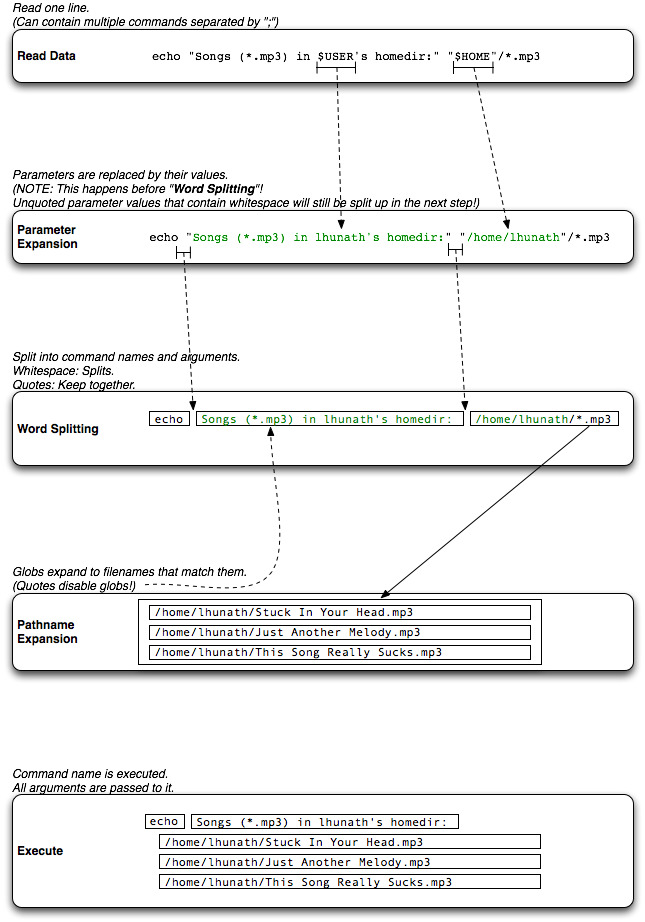
\includegraphics[width=.8\textwidth]{bash-parser}
  \caption{Bash Parser}
  \label{fig:bash-parser}
\end{figure}

Figure \ref{fig:bash-architecture} is a
\href{http://aosabook.org/en/bash.html}{better presentation}. From
which, we find \textit{expansion} plays a critical role in the
whole procedure.

\begin{figure}
  \centering
  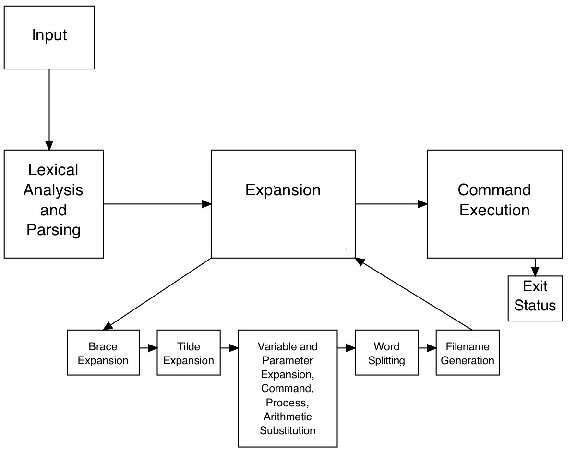
\includegraphics[width=.8\textwidth]{bash-architecture}
  \caption{Bash Architecture}
  \label{fig:bash-architecture}
\end{figure}

Basically, the parser carries out the following procedures:

\begin{enumerate}
\item Read script source line by line. For each line, 
\item Process quotes.
\item Split a line into commands. For each command,
\item Process redirections and brace expansions.
\item Perform expansions, including parameter expansion,
  comamnd/process/arithmetic substitution etc.
\item Word Splitting: split the command into command name and arguments list.
\item Execute the command.
\end{enumerate}

\section{Command History}
\label{sec:command-history}

Bash provides command-line tools for editing and manipulating
command history. Check the \uline{HISTORY EXPANSION} as per the
man
page. \href{https://samrowe.com/wordpress/advancing-in-the-bash-shell/}{Advancing
  in the Bash shell} is an excel tutorial.

One of the those is \lstinline|history|, listing previously
executed Bash commands. \lstinline|fc| is the counterpart for Sh
shell.

There exist a list of internal variables related to history
commands, like:

\begin{lstlisting}
$HISTCMD $HISTFILESIZE !N !-N !! !$ 
\end{lstlisting}

Especially, \lstinline|!!| is a synonym for
\lstinline|!-1|. \lstinline|!$| expands to the last word of the
preceding command. Usually, it will the the last argument.

Generally, we have \uline{Event Designator} that select a command
from history, \uline{Word Designator} that select a \textit{Bash
  word} from the selected command, and \uline{Modifiers} are a
sequence of modifiers to adjust the selected command. An event
designator starts with the exclamation mark \uline{!} .

One of the most useful modifier is \textit{p} that print but not
execute the selected command.

\section{Code Disassembling}
\label{sec:bash-code-disassembling}

I think it is a good practice to retrospect what have been learned
recently, reviewing progress and summarize
experience. Additionally, I'd like to make use of such chances to
format the knowledge in my own wording. Such an \textit{output}
process testifies whether knowledge settles down and consolidates.

This section disassembles the \verb|missTime| code line by
line. Especially, I should explain \textit{how} and
\textit{why}. The complete code is attached at
\ref{sec:bash-misstime}.

\section{Quoting}
\label{sec:bash-quoting}

Quoting is used to remove the special meaning of certain
characters (i.e. whitespace for word splitting) or words to the
shell. For example, it prevents reserved words from being
recognized as such. It can also prevent parameter expansion.

There exist multiple quoting mechanism, namely:

\begin{itemize}
\item the escape character \verb|\|
\item single quote
\item double quote
\item ANSI-C quote
\end{itemize}

A non-quoted \textbackslash{} preserves the literal meaning of the
next character, with the exception of newline. \verb|\newline| is
treated as a line continuation like

\begin{lstlisting}
echo \
'hello, world'

echo 'hello,
world'
\end{lstlisting}

For quotes, there is no need to append the trailing backslash. The
newline splits the string into two lines.

Single quotes preserve the literal meaning of each character
within the quotes, except single quote (even preceding by a
backslash which also preserves its literal meaning) like:

\begin{lstlisting}
echo 'what\'s your name?'
\end{lstlisting}

The backslash does not serves as escape. This is an illegal Bash
statement and it actually is parsed as three parts, namely
\lstinline|<what\>|, \lstinline|<s your name?>| and the final
apostrophe \verb|'|. The second part is not quoted and the third
single quote is unbalanced and Bash expects another single
quote. The revised versions are legal but may not be our desired
results.

\begin{lstlisting}
echo 'what\'s your name?
echo 'what\'s your name?'jim'
\end{lstlisting}

But if we \lstinline|printf '\n'|, a newline is correctly
printed. Why? That is because \verb|\n| is literally passed the
the command \verb|printf|. It is the responsibility of
\verb|printf| to interpret \verb|\n| as newline. For Bash, they
are just a backslash \verb|\| and character \verb|n|, not a
newline.

Apparently, single quotes is kind of \textit{strong} quoting
method to preserve character meaning. But we can precede it by
backslash \$ to preserve the escaping ability of \textbackslash{},
where escaped characters are replaced by their
\href{https://www.gnu.org/software/bash/manual/bash.html#ANSI_002dC-Quoting}{ANSI-C
  Quoting}. For example,
\lstinline|$'\t\''| presents a horizontal tab and a single quote
itself. Therefore, if we want to include a literal single quote
within singles qoutes, we can precede the quotes with dollar
\lstinline|$|.

Double qoutes is somewhat relatively flexible. It preserves the
literal meaning of all characters, except that of
\lstinline|$|, \lstinline|`|, \lstinline|\| etc. Within double
quotes, \textbackslash{} can be used to escape \lstinline|$|,
\lstinline|"|, \lstinline|`|, \lstinline|\| and
\verb|newline|. For example,

\begin{lstlisting}
echo "looooooooooooooooooooooooooooooooooooooooooooooooooooooooooooooooong\
,line. \$"

echo 'looooooooooooooooooooooooooooooooooooooooooooooooooooooooooooooooong\
,line. \$'
\end{lstlisting}

A double-quoted string preceded by a dollar sign
\lstinline|$"string"| will cause the string to be translated
according to the current \textit{locale}.  If the current locale
is C or POSIX, the dollar sign is ignored.  If the string is
translated and replaced, the replacement is
double-quoted. Attention, this is not parameter expansion, nor
ANSI-C quoting.

\section{printf and echo}
\label{sec:printf-echo}

\begin{lstlisting}
printf 'Usage: ./missTime <number-of-test> <input-file>\n\n'
\end{lstlisting}

Use Bash's built-in or system's \lstinline|printf| instead of
\lstinline|echo|. \lstinline|printf| supports all C language
format to allow flexible output. For instance, We can use it to
assign variables by \lstinline|-v| option:

\begin{lstlisting}
printf -v var "hello, world\n"; declare -p var
\end{lstlisting}

To check Bash's \lstinline|printf|, just run
\lstinline|help printf|. My Gentoo's system version is located at
\lstinline|/usr/bin/printf| that is part of GNU coreutils. In
terminal emulator, \lstinline|type -a printf| lists both
versions. Unlike \lstinline|echo|, \lstinline|printf| does not
append a \textit{newline} by default.

For the full contention, check
\href{https://unix.stackexchange.com/q/65803/74407}{Why is printf
  better than echo?} and
\href{https://wiki.bash-hackers.org/commands/builtin/echo}{echo
  protability considerations}.

As the page writes, \textit{never use options/arguments to echo}
like \verb|-e|. Also, do not use it to print \textit{uncontrolled
  data} such as external input (filename, arguments etc. from user).

In summary, \lstinline|printf| is far more reliable and safer. It
litterally output as the format specifies.

A final note, to output sequential dashes like \verb|---|,
\lstinline|printf| can do as follows:

\begin{lstlisting}
printf -- '---\n'
printf '%s\n' "---"
printf '---\n' # error
\end{lstlisting}

For the principle behind, just read Bash manual, the OPTIONS
section. Basically, everything after two consecutive dashes is
treated as arguments (i.e. filenames). In other words, it signals the
end of command options and disable further option processing.

Command \lstinline|tee -a| writes to both standard output and
files, which can be combined with \lstinline|printf| like:

\begin{lstlisting}
printf '%s\n' "hello, world" | tee -a file.txt
\end{lstlisting}

Single quotes are preferred in the format part unless you want
parameter expansion there.

Let's have a look at another sample:

\begin{lstlisting}
printf '%s\n' '1d' w | ed -s "$_full"

sed -i -e '1d' "$_full"
\end{lstlisting}

You will find there is only one format specification \verb|%s| but
two arguments \verb|'1d'| and \verb|w| (not quoted). In such case,
the format specifiers are reused:

\begin{quotation}
  The format is re-used as necessary to consume all of the
  arguments. If there are fewer arguments than the format
  requires, extra format specifications behave as if a zero value
  or null string, as appropriate, had been supplied.
\end{quotation}

\section{Exit Codes and Boolean}
\label{sec:exit-codes-boolean}

\begin{lstlisting}
[[ "$1" == @(-h|--help) ]] && exit 0
\end{lstlisting}

\lstinline|exit| terminates the current shell \textit{process}
while \lstinline|return| just terminates a \textit{function}
execution.

Both give numeric \verb|0| for success execution and other
specific codes for different error types. Here is a list of Bash
\href{http://tldp.org/LDP/abs/html/exitcodes.html#EXITCODESREF}{Reserved
  Exit Codes}.

The relation between Shell exit codes and boolean is as follows:
\textit{exit and return codes are just numeric integers}. They are
not boolean values. To be logically consistent, we should
correctly interpret the integer codes.

Bash treats 0 for true while others (1 included) for
false. Numeric 1 is just one instance among the whole set of
failure codes. It is not what we might think that false is bound
to 1. Let's have a closer look at the procedure.

A sub-shell decides the status of execution. If a desired
outcome is captured, it is logically true/successful. Otherwise,
different failure outcomes are treated as false.

Unpon successful execution, numeric 0 is returned back to the
parent process. Actually, any number could be returned to
represent
\href{https://stackoverflow.com/a/21439109/2336707}{successful
  execution}, but as the link points out 0 is \textit{platform and
  encoding independent}.

Now that numeric 0 is returned for success and other numerics for
failure, the caller or the topmost Bash process should correctly
interpret numeric codes to boolean true/false when \lstinline|if|,
\lstinline|[[ ]]|, or \lstinline|while| are involved.

Attention that, \textit{true} and \textit{false} are not
\href{https://www.gnu.org/software/bash/manual/html_node/Reserved-Word-Index.html}{reserved
  words} in Bash. But we have commands
\lstinline|type -a true false|. Up to now, you may find, many
commands has two versions: one from GNU coreutils and the other
from Bash builtins.

To test if a command is successfully executed, just test the command:

\begin{lstlisting}
if command ; then : ; fi
\end{lstlisting}

The next code also works, but it is \textit{stupid}. It runs a new
command \lstinline|[[| to test another command's exit code.

\begin{lstlisting}
# -or-
command; if [[ $? -eq 0 ]]; then : ; fi
\end{lstlisting}

Here, we find another command pair \lstinline|type -a [|.
\lstinline|[[| is only available to Bash.

\section{read}
\label{sec:bash-read}

\begin{lstlisting}
read -r _ _ _ _ip _ < <(ip -4 -o addr show scope global dev bond0)
 _ip="${_ip%/*}"
\end{lstlisting}

\lstinline|read| is another Bash builtin that read a line from
standard input and split it into fields based on \lstinline|IFS|
\begin{cprotect}
  \footnote{The default Internal Field Separator is <space>,
    <tabular>, and <newline>, namely \lstinline|$' \t\n'|.}
\end{cprotect}. Check details at
\href{https://www.gnu.org/software/bash/manual/bash.html#Word-Splitting}{Word
  Splitting}. You are recommended to include the \lstinline|-r|
argument as it disables bachslash escape.

\lstinline|read| assigns the first splitted word to the first
name, the second word to the second name and so on, with any
leftover words assigned to the last name.

Why are there \textit{underscore}s before and after
\lstinline|_ip|? Mainly, they are just placeholders to skip
unwanted splitted words, explained in the next section.

Thus, the first three undersocres capture the three words
ahead while the last underscore captures everything else, including the
IFS characters and leaving the remaining part untouched.

Attention that, \lstinline|read| uses \verb|IFS| as \textit{field}
separator while use \lstinline|-d| as \textit{record} separator.

\subsection{readonly}
\label{sec:bash-readonly}

The builtin \lstinline|readonly| command with the form

\begin{lstlisting}
readonly [-aAf] [name[=value] ...]

readonly -p
\end{lstlisting}

marks each \textit{name} as \textit{readonly}. if a \textit{value}
is supplied, do assignment before marking as read-only.

\section{Special Parameters}
\label{sec:bash-special-parameters}

These parameters may \textit{only be referenced}; assignment to
them is not allowed. Let's see how them are expanded.

\begin{itemize}
\item \verb|*|: \lstinline|$*| expands to positional
  parameter. Without double quotes, each positional parameter
  expands to a separate word. Within double quotes, all positional
  parameters expand to a single word with the value of each
  positional parameter separated by the first character of
  variable \lstinline|IFS|.
\item \verb|@|: \lstinline|$@| is similar to \lstinline|$*|,
  except that when in double quotes, each positional parameters
  also expand a separate word.
\item \verb|#|: \lstinline|$#| expands to the number of positional
  parameters in decimal.
\item \verb|?|: \lstinline|$?| expands to the exit status of the
  most recently executed \textit{foreground} pipeline.
\item \verb|-|: \lstinline|$-| expands to the current
  \textit{option} flags as specified upon invocation, by the
  \lstinline|set| builtin command, or those set by the shell
  itself (such as \lstinline|bash -i|).
\item \verb|$|: \lstinline|$$| expands the process ID of the
  \textit{topmost} shell. In a sub-shell (i.e. \lstinline|( )|, it
  expands the process ID of the invoking shell (upper level) as it
  is \textit{inherited}. In a sub-shell, use \lstinline|BASHPID|
  instead, which expands to the process ID of \textit{current}
  shell.
  \lstinline|echo $$ $BASHPID; ls -l /proc/self; (echo $$ $BASHPID; ls -l /proc/self)|.
  Also check
  \href{https://unix.stackexchange.com/a/333227}{/proc/self}.
\item \verb|!|: \lstinline|$!| expands to the process ID the
  \textit{job} most recently placed into the background.
\item \verb|0|: \lstinline|$0| expands to the name of shell or
  shell script.
\item \verb|_|: \lstinline|$_| expands to the last argument of
  privous simple command. Read the next section.
\end{itemize}

\section{Underscore}
\label{sec:bash-underscore}

Firstly, Bash regards \textit{underscore} \lstinline|_| as
\href{https://www.gnu.org/software/bash/manual/bash.html#Special-Parameters}{special
  parameter}. Meanwhile, it is a standalone legal \textit{name}
(vairable) and can be part of a variable as well. In short, it is
the \uline{only} \textit{parameter} that is also a valid
\textit{variable name}.

\begin{lstlisting}
echo 'hello, world'
declare -p _ ; declare -p _
\end{lstlisting}

As a special parameter, the value of undersocre \verb|_| is
assigned \textit{automatically} by Bash process as depicted in the
next section, namely \textit{expansion}
\ref{sec:bash-parameter-expansion}. At the very beginning, it is
set to the absolute \textit{pathname} of the shell or script
file. Subsequently, \textit{expand}s to the last argument of
previous simple command.

Though it is a variable, we can \textbf{not} assign value to it
explicitly. In other words, assignment to it is legal but in vain.

\begin{lstlisting}
_="a"
declare -p _
\end{lstlisting}

That is the reason we use it as a placeholder for \lstinline|read|
command. Its value is \textit{unstable} and got \textit{overriden}
immediately after each Bash command. Values assigned to it take no
effects. We can verify this behavior by:

\begin{lstlisting}
read -r _ var <<< 'hello, world'
declare -p _
# -or-
printf '%s\n' "$_"
\end{lstlisting}

The code outputs \lstinline|declare -- _="var"| since the last
argument of \lstinline|read| is a name (\verb|var| here).

Pay attention to the difference between \textit{declare} (only the
name is required) and \textit{printf} (name should be expanded by
\lstinline|$|).

\section{globstar}
\label{sec:bash-globstar}

The special glob character \lstinline|*| matches any string of any
length, including the \textit{null} string.

When the \lstinline|shopt -s globstar| option is enabled, two
ajacent two adjacent \lstinline|*|s used as a single pattern will
match all files and zero or more directories and subdirectories.
If followed by a \lstinline|/|, two adjacent \lstinline|*|s will
match only directories and subdirectories.

\textit{globstar} is also called \textit{recursive glob}.

\section{extglob}
\label{sec:bash-extglob}

Here are a few \textit{extglob} samples. To turn on this Bash
feature, just \lstinline|shopt -s extglob| \textit{on a newline}.

\lstinline|extglob| changes the way certain characters are
parsed. It is
\href{https://mywiki.wooledge.org/glob#extglob}{necessary to have
  a newline} (\textbf{not} just a semicolon) between
\lstinline|shopt -s extglob| and any subsequent commands to use
it. This is because the command line is parsed before
\lstinline|shopt| command is evaluated. Check the parser section
before.

Likewise, you cannot put \lstinline|shopt -s extglob| inside a
statement block that uses extended globs, because the block as a
whole must be parsed when it's defined; the \lstinline|shopt|
command won't take effect until the block is evaluated, at which
point it's too late. In fact as Bash parses the entire statement
block before evaluating any of it, you need to set
\textit{extglob} outside of the outermost block.

The first example below, does not turn on \lstinline|extglob|
correctly and report error.

\begin{minipage}{1.0\linewidth}
\begin{lstlisting}
shopt -u extglob
shopt -s extglob ; touch foo bar ; echo @(foo|bar)
# -bash: syntax error near unexpected token `('

_ip=127.0.0.1 _std_array[6]="https://www.baidu.com/a/b/c/d?v=k"
printf '%s\n' "${_std_array[6]}"
shopt -q extglob; _extglob_set=$?
(( _extglob_set )) && shopt -s extglob
_delete_url=${_reply_array[X-True-Cache-Key]#http?(s)://}
(( _extglob_set )) && shopt -u extglob

bash -c $'shopt -u extglob\nshopt -s extglob ; 
url="https://www.google.com/a/b/c" ;
_delete_url=${url#http?(s)://} ;
shopt -u extglob; printf "%s\n" "${_delete_url}"'

shopt -u extglob
var='--help' ; [[ "$var" == @(-h|--help) ]] && echo 'yes'
\end{lstlisting}  
\end{minipage}

The second case replaces the \lstinline|://host/| with
\lstinline|://ip/|, which combines the features of
\textit{extglob} and \textit{parameter expansion} in the form
\lstinline|${parameter/pattern/string}|. In the pattern part, we
should escape the backslash \textbackslash while in the string
part, leave as it is since this part is leterally substituted.

The next two cases show both
\lstinline|${parameter/pattern/string}| and \verb|[[| use
\lstinline|extglob| internally even we turn it off.

But to be consistent and robust, we are still recommended to put
it on separate lines. This rule applies to other shell options as
well.

\section{Process Substitution}
\label{sec:bash-process-substitution}

Still the same code snippet at previous section, we have

\begin{lstlisting}
< <(ip -4 -o addr show scope global dev bond0)
\end{lstlisting}

\lstinline|>(list)| and \lstinline|<(list)| are called
\href{https://www.gnu.org/software/bash/manual/bash.html#Process-Substitution}{Process
  Substitution} \textit{operator}s that allow a process's input or
output to be referred to using a \uline{filename}, which the
process get inputs from or output results to a file. Attention, a
sub-shell is spawned when process substitution happens (there is a
pair of parentheses there).

The keyword \textit{list} here may be a normal command or a
pipeline of commands. No space may appear between the \verb|<,>|
and the left parenthesis \verb|(|, otherwise the form would be
interpreted as a redirection.

The operators execute commands in \textit{list} in a sub-shell
and send the output to a file. The operator is then substituted
with the pathname of that file. Process Substitution is supported
on systems that support
\href{http://mywiki.wooledge.org/NamedPipes}{named pipes} (FIFOs)
or the \verb|/dev/fd/| method of naming opened files. We can just
think of the two forms as just filenames, which is done by giving
the list a name in the filesystem:

\begin{quotation}
  process substitution = filename
\end{quotation}

For the input form \lstinline|>(list)|, writing to the file will
provide input for the enclosed \textit{list} like:

\begin{lstlisting}
# command ... >(list) ...

echo >(true)

cat file.txt > >(wc -l)
\end{lstlisting}

The first example displays filename of the command
substitution. The second \textit{redirects} the output of
\lstinline|cat| to the input filename.

If the output form
\lstinline|<(list)| is used, the file can be read to obtain the
output of the \textit{list} like:

\begin{minipage}{1.0\linewidth}
\begin{lstlisting}
# command ... <(list) ...

echo <(true) # print the output filename
cat <(list)  # print the contents of the output filename

# compare the two output filenames
comm -3 <(sort a.txt | uniq) <(sort b.txt | uniq)
\end{lstlisting}
\end{minipage}

Back to the beginning code, the leftmost \verb|<| is a normal I/O
redirection, meaning read from the process substitution. Pay
attention to the extra space between the two \verb|<|, otherwise
it would be a
\href{https://www.gnu.org/software/bash/manual/bash.html#Here-Documents}{Here
  Document}.

\section{Parameter Expansion}
\label{sec:bash-parameter-expansion}

\begin{lstlisting}
_num_of_tests=${1:-10}
\end{lstlisting}

The purpose of this code is to assign value to
\verb|_num_of_tests| from either user input or the default
\verb|10|.

The special \$ symbol of Bash introduces \textit{parameter
  expansion}, \textit{command substitution}, or \textit{arithmetic
  expansion}. The terminology - \textit{parameter} - is defined in
the manul, please have a read. To put it simple, parameter is an
entity that stores values, it can be a \textit{name}, a
\textit{number}, or
\href{https://www.gnu.org/software/bash/manual/bash.html#Special-Parameters}{special
  parameters} like \verb|* @ # _| etc., of the list, undersocre is
explained in a prior section.

\textit{name} is what we usually call as \textit{varaible} or
\textit{function name}. Also referred to as an
\textit{identifier}.

The parameter symbol to be expanded may be enclosed in braces
which are \textit{optional} but \textit{safer} as braces separate
the variable from characters immediately following it.

The basic form is
\lstinline|${parameter}|. Our case is
\lstinline|${parameter:-word}| that means the expansion of
\textit{word} is substituted if \textit{parameter} is null or
unset, otherwise the value of \textit{parameter} is substituted.

Here are three extra examples:

\begin{minipage}{1.0\linewidth}
\begin{lstlisting}
for f in full real; do declare "_$f"="${_log_time}-${_num_of_tests}-$f.log"; done
for f in "${_full}" "${_real}"; do echo -n >| "$f"; done  
\end{lstlisting}
\end{minipage}

This code uses \lstinline|echo -n| to create an empty new
file, which can also be accomplished by \lstinline|touch| or
\lstinline|printf ''|

\section{Brace Expansion}
\label{sec:brace-expansion}

\href{https://wiki.bash-hackers.org/syntax/expansion/brace}{Brace
  expansion} is used to generate arbitrary \uline{strings}. It
takes the following forms:

\begin{lstlisting}
# {string1,string2,...,stringN}
{a,b,c,d}
# {<START>..<END>}
{1..10}
# {<START>..<END>..<INCR>} (Bash 4)
{1..10..2}
# <PREAMBLE>{........}
# {........}<POSTSCRIPT>
# <PREAMBLE>{........}<POSTSCRIPT>
a{b,c,d,}.txt
\end{lstlisting}

Both the PREAMBLE and POSTSCRIPT parts are optional. The last
example above can expand to \verb|a.txt| for the trailing
comma \lstinline|,|.

Within the braces, we can place either a series of comma-separated
strings, or a \textit{sequence expression}. The should be
\textit{no} space between the list elements. Results of expanded
strings are not sorted; let to right order is preserved.

A sequence expression takes the form \lstinline|{x..y[..incr]}|,
where \lstinline|x| and \lstinline|y| (both inclusive) are either
intergers or single characters, and \lstinline|incr|, an optional
argument, is an integer. Both \lstinline|x| and \lstinline|y| must
be of the same type.

Supplied integers may be prefixed with 0 to force each term to
have the same width like
\lstinline|for i in {01..12}; do echo $i; done|.

It is different to
\href{https://www.gnu.org/software/bash/manual/bash.html#Filename-Expansion}{globbing}
that matches \uline{filenames} by default (unless used in
parameter expansion).

\begin{quotation}
  This mechanism is similar to pathname expansion, but the filenames generated \textbf{need not exist}.
\end{quotation}

That means \lstinline|{foo,bar}.txt| expands to
\lstinline|foo.txt| and \lstinline|bar.txt|. Whether the two
strings are used as filenames or not depends on how you use it.

\begin{lstlisting}
for f in {foo,bar}.txt ; do echo "$f" ; ls "$f" ; done
\end{lstlisting}

But glob \lstinline|*.txt| only expands to \textit{existing} files. If
no files are matched, it expands to the glob itself unless
\lstinline|nullgob| is enabled which makes it expands to
\textit{null string}.

\begin{lstlisting}
bash -c $'shopt -u nullglob\nfor f in *.txt; do ls "$f"; done'

bash -c $'shopt -s nullglob\nfor f in *.txt; do ls "$f"; done'
\end{lstlisting}

From section Bash Parser \ref{sec:bash-parser}, we know brace
expansion happens before all the rest expansions. Any characters
special to other expansions are preserved in the result:
\textit{strictly textual}. So brace expansion makes

\lstinline|echo {a,b}$PATH|

be

\lstinline|echo a$PATH b$PATH|

before \verb|PATH| is parameter-expanded.

Similarly, a brace expansion with range like \lstinline|{1..200}|
can not be expressed like:

\begin{lstlisting}
a=1 b=200
echo {$a..$b}
\end{lstlisting}

Actually such code does not satisfy a legal barce expansion
requirement. Within the \textit{unquoted braces pair}, there
should be \textit{at least} a comma or a sequence expression.The
textual \verb|$a| and \verb|$b| (not parameter-expanded), the dots
inbetween included, neither contains a comma nor are sequence
expression. Hence, during the brace epxansion phase, the code is
ignored. When it comes to the parameter expansion, it becomes a
single string \lstinline|{1..200}|.

Brace construction is normaly used when the common prefix or
suffix of strings to be generated are much longer:

\begin{lstlisting}
mkdir /usr/local/src/bash/{old,new,dist,bugs}
#
chown root /usr/{ucb/{ex,edit},lib/{ex?.?*,how_ex}}
#
echo {{A..Z},{a..z}}
#
echo {A..Z}{0..9}
\end{lstlisting}

You will find from the code, brace expansion can be nested. It
also supports concatenation.

\section{Parameter Transformation}
\label{sec:bash-param-transf}

\begin{lstlisting}
printf 'curl -ksSI '
# 4.4
printf -- '-H %s ' "${_headers_array[@]@Q}"
printf -- '-H %s --resolve %s %s\n\n' "x-c3-debug:enabled" "${_resolve@Q}" "${_url@Q}"

# < 4.4
printf -- '-H %q ' "${_headers_array[@]}"
printf -- '-H %q --resolve %q %q\n\n' "x-c3-debug:enabled" "${_resolve}" "${_url}"
\end{lstlisting}

Since \href{http://mywiki.wooledge.org/BashFAQ/061}{Bash 4.4},
\uline{parameter transformation} is supported in the form
\lstinline|${parameter@operator}|. Of the operators, \verb|Q|
expands the parameter as a string that is the value of parameter
quoted in a format that can be reused as input like
\lstinline|ar=(a 1 "b ; c") ; printf '%s\n' "${ar[@]@Q}"|.

Before Bash 4.4, we can resort to \lstinline|printf '%q'| which
quotes the argument in a way that can be reused as shell input.

\section{regex Test}
\label{sec:bash-regex-test}

\begin{lstlisting}
_headers_regex=$'\^\~\$headers=\'(.*)\)@\|#\(\''
_headers_regex='\^\~\$headers='\''(.*)\)@\|#\('\'

_https_regex='^https://'
[[ "${_int_log}" =~ $_regex ]] && printf '%s\n' "${BASH_REMATCH[1]}"
\end{lstlisting}

Bash support the
\href{http://mywiki.wooledge.org/RegularExpression}{extended
  regular expression} by \textit{conditional command} \verb|[[|
with binary operator \verb|=~|.

If the pattern is properly matched, results is assigned to
built-in variable \lstinline|BASH_REMATCH|. It is an array
variable with index 0 the portion of the string matching the
entire regular expression (the complete match, \textbf{not} the
whole string). The element with index \textit{n} is the portion of
the string matching the \textit{n}th parenthesized sub-expression
(capture group). If there are nested parenthesis level, the inner
index is that of the outer level plus 1.

\lstinline|BASH_REMATCH| is \textit{read only}. We cannot change
its value. Usually, just assign it to a temporary variable.

Pay attention the two methods to define the regular
expression. The first one is preceded by a
\verb|$| within which \verb|\'| is correctly interpreted. While
the 2nd version, put the \verb|\'| outside of single
quotes\verb|'foo-bar'|.

\section{Array}
\label{sec:bash-array}

Bash provides one-dimentional \textit{indexed} and
\textit{associative} array variables. The \textit{declare} builtin
can explicitly declare an array:

\begin{lstlisting}
declare -a indexed_array # optional
declare -A associative_array=()
\end{lstlisting}

Indexed array can be any vairable, and hence a declaration is
optional.

\begin{quotation}
  Any reference to a variable using a valid subscript is legal,
  and bash will create an array if necessary.
\end{quotation}

On the contrary, associative array \textit{must} be
declared before usage.

Indexed arrays are zero-based while associative array resembles
Python \textit{dictionary}, with key and value pairs stored. Pairs
are not sorted.

When assigning elements to an array, please enfold the
\textit{subscript} with square brackets.

\begin{lstlisting}
indexed_array[0]=12
indexed_array=( [1]='a' 'b' 'c' )
printf '%s\n' "${indexed_array[@]}"
#
declare -A associative_array=( ['addr']='usa' )
associative_array['name']='jim'
associative_array=( ['age']=30 )
for key in "${!associative_array[@]}"; do printf '%s: %s\n' "$key" \
"${associative_array[$key]}"; done
\end{lstlisting}

Array elements can be referrenced by the form
\lstinline|${name[subscript]}|. The curly braces are required to
avoid conflicts with filename expansion operators.

\begin{quotation}
  \lstinline|${|. Without curly braces parameter expansions refer
    to the \textit{longest valid variable name} or
    \textit{shortest positional parameter}.
    \lstinline|"${var}bar"| expands the parameter named
    \textit{var} while \lstinline|"$varbar"| expands
    \textit{varbar}.
    \lstinline|"$123"| references \lstinline|argv[1]| and
    \lstinline|"${123}"| references \lstinline|argv[123]|. Braces
    are requried for positional parameters \uline{> 9},
    \uline{special PEs}, and \uline{array expansions}:
    \lstinline|${10}|, \lstinline|${var##pat}|,
    \lstinline|${arr[5]}|. BRACES AREN'T A SUBSTITUTE FOR QUOTES!
  \end{quotation}

If the \textit{subscript} is
omitted, \lstinline|$name| implies a subscript of zero \verb|0|,
which suggests \textit{name} is an indexed array or an associative
array with a key of zero \verb|0|.

\begin{lstlisting}
unset ar; declare -A ar=( [0]=a ["hello"]=1 )
declare -p ar; printf '%s\n' "$ar"
[[ -v ar ]] && echo "yes"
\end{lstlisting}

To print array:

\begin{lstlisting}
# indexed array
printf '%s\n' "${idexed_array[@]}"
# associative array
for key in "${!idexed_array[@]}"
do
    printf '%s: %s\n' "$key" "${idexed_array[$key]}"
done
\end{lstlisting}

The code above uses special subscript \lstinline|@| that expands
to positional parameter. Another special subscript is
\lstinline|*|, when double quoted, expanding to a single word with
each element separated by the first character of the
\lstinline|IFS| which by default is \textit{space}. Hence:

\begin{enumerate}
\item For printing, use \lstinline|@| instead of \lstinline|*|
  unless explicitly required.
\item When setting custom \lstinline|IFS|, pay attention to the
  character sequence.
\end{enumerate}

Now, let's have a look at the following code:

\begin{lstlisting}[caption={curl CRLF},label={lst:curl-crlf}]
declare -A _reply_array=()
while IFS=' :' read -r key value
do
    [[ -n "$key" && "$key" != [[:space:]] && "$key" != + ]] || continue
    _reply_array[${key,,}]=${value%$'\r'}
done < "curl-reply.log"
\end{lstlisting}

\begin{enumerate}
\item Associative array must be delcared.
\item The first character of \lstinline|IFS| is set to space.
\item \lstinline|-r| argument of \lstinline|read| is adopted.
\item \lstinline|continue| starts the next loop instantly.
\item \textit{key} is transferred to lower case by parameter
  expansion in the form
  \lstinline|${parameter,,pattern}|. \textit{pattern} is omitted.
\item Remove trailing \textit{carriage return} \lstinline|\r| from
  \lstinline|curl|.
\end{enumerate}

The sixth item is really hostile to programmers. Basically,
\lstinline|curl| feeds back messages with
\href{https://stackoverflow.com/a/30957952/2336707}{CRLF}
instead of \lstinline|\n|. We can check this by
\lstinline|sed -n l|. To reuse some returned headers, we should
firstly
\href{https://stackoverflow.com/a/35019553/2336707}{remove} the
extra \lstinline|\r|.

\section{Command Substitution}
\label{sec:bash-command-substitution}

Similar to Process Substitution
\ref{sec:bash-process-substitution} above,
\href{https://www.gnu.org/software/bash/manual/bash.html#Command-Substitution}{command
  substitution} performs the expansion by executing the command
within a sub-shell.

It allows the output of a command to substitute the command
itself, with trailing newlines delete. We can just think of
command substitution as a string and using the output of a command
as an argument. No filenames are involved.

It takes the following two
forms. The \textit{backquote} form is deprecated and discouraged.

\begin{lstlisting}
$(command)

`command` # deprecated
\end{lstlisting}

If the substitution appears within double quotes like
\lstinline|"$(command)"|, \textit{word splitting} and
\textit{filename expansion} are not performed on the results,
which is a \textit{preferred} method.

Command substitution is useful when we want to assign a command
output to a variable like \lstinline|_date="$(date -Idate)"|.

The command substitution \lstinline|$(cat file)| can be replaced
by the equivalent but faster
\lstinline|$(< file)| (without sub-shell). The later one is a
\textit{specical} case of command substitution. It does not invoke
any command and Bash just substitutes it with the contents of
file.

\section{Assignment and Simple Command}
\label{sec:assignm-simple-comm}

\begin{lstlisting}[basicstyle=\tiny\ttfamily]
IFS=$'\n' _log_array=( $( awk -F'[[:space:]]*\\)@(in|out)#\\([[:space:]]*' \
                              '{ for (i = 1; i <= NF; ++i) print $i; }' <<< "${line}" ) )
# better
mapfile -t _log_array < <( awk -F'[[:space:]]*\\)@(in|out)#\\([[:space:]]*' \
                              '{ for (i = 1; i <= NF; ++i) print $i; }' <<< "${line}" )
#
IFS=';' read -ra _headers_array <<< "${BASH_REMATCH[1]}"
_headers_array=( "${_headers_array[@]/#/-H}" )
\end{lstlisting}

In the first assignment uses \lstinline|awk| command substitution
with output assigned to an indexed array directly. This
substitution is not double-quoted, so word splitting and pathname
expansion happens before assignment. The second assignment uses
\lstinline|awk| process substitution and mapfile
\ref{sec:bash-mapfile} (explained in a standalone section), which
is much \textit{faster} and \textit{safer} method.

Why, in this section, I want to talk about assignment and simple
command? We can think of
\href{https://www.gnu.org/software/bash/manual/bash.html#Simple-Commands}{simple
  command} as just a command name followed by its arguments. From
\href{https://www.gnu.org/software/bash/manual/bash.html#Simple-Command-Expansion}{Simple
  Command Expansion}, we find:

\begin{quotation}
  If no command name results, the variable assignments affect the
  current shell environment. Otherwise, the variables are added to
  the environment of the executed command and do not affect the
  current shell environment. If any of the assignments attempts to
  assign a value to a readonly variable, an error occurs, and the
  command exits with a non-zero status.
\end{quotation}

The only command \lstinline|awk| is executed in a sub-shell, The
two assignments
\lstinline|IFS=$'\n' _log_array=| affect the current shell. That
is to say, from here on, the new \lstinline|IFS| value is changed
for the whole Bash process. Instead, the \lstinline|IFS|
associated with the \lstinline|read| statement only affects the
\lstinline|read| command itself.

Let's reformat the code like:

\begin{lstlisting}[basicstyle=\tiny\ttfamily]
IFS=$'\n'
_log_array=( $( awk -F'[[:space:]]*\\)@(in|out)#\\([[:space:]]*' \
                    '{ for (i = 1; i <= NF; ++i) print $i; }' <<< "${line}" ) )
IFS=$' \t\n'
\end{lstlisting}

It becomes more understandable and more clearer.

\paragraph{Extra notes}: \subparagraph{} Recall that indexed array
can be declared by \lstinline|-a| argument. \lstinline|read|
command supports reading into an indexed array by the same
argument.  \subparagraph{}
\lstinline|"${_headers_array[@]/#/-H}"| is another example of
parameter expansion in the form
\lstinline|${parameter/pattern/string}|. It inserts \lstinline|-H|
in front of each array element.

\section{Commands}
\label{sec:bash-commands}

\subsection{sed}
\label{sec:bash-sed}

\lstinline|sed|, as described in the manual, is a stream editor
for filtering and transforming text.

We can use it to delete empty lines:

\begin{lstlisting}
sed -i.bak '/^[[:space:]]*$/d' file.txt
sed -i.bak '/[^[:space:]]/!d' file.txt
\end{lstlisting}

The \lstinline|-i[SUFFIX]| or \lstinline|--in-place[=SUFFIX]|
option edits files in place (makes backup if SUFFIX supplied).

Form \lstinline|/regexp/| matches lines against the regular
expression. In the example above,
\lstinline|^[[:space:]]*$| matches empty lines. The traling
command \lstinline|d| means to delete matched lines.

To support extended regular expressions, add option
\lstinline|sed -r| like:
\lstinline|sed -r 's/[[:blank:]]+/ /g' /proc/slabinfo|. Otherwise,
the plus symbol should be escaped like:
\lstinline|sed 's/[[:blank:]]\+/ /g' /proc/slabinfo|.

The variant version is somewhat not so obvious but usually faster
if the file has less empty lines. Pay attention to the exclamation
mark \lstinline|!| before command \lstinline|d|. This version
means as long as a non-space character is matched, don't delete
the line.

Another useful form is \lstinline|s/regexp/replacement/| that
matches file lines agaist the \textit{regex} and \textit{replace}s
the matched parts with \textit{replacement}. We can use
\lstinline|&| in the \textit{replacement} to represents the
matched parts like \lstinline|s/hello/=&=/| means to enclose
string \textit{hello} with symbol \verb|=|.

The snippet below replaces \textit{google} with \textit{bing} if
the URL contains \textit{foo}. Note that in the regular expression
part, dot should be escaped while in the replacement part
\textit{not}. A version with \lstinline|awk| are also provided for
reference. Please read more in \verb|awk| section.

\begin{minipage}{1.0\linewidth}
\begin{lstlisting}
var=$'https://www.google.com/foo?v=xyz\nhttp://www.baidu.com/bar?v=uvw\n'
printf '%s\n' "$var"
sed '/foo/s/www\.google\.com/www.bing.com/' <<< "$var"

var=$'https://www.google.com/foo?v=xyz\nhttp://www.duckduckgo.com/bar?v=uvw\n'
printf '%s\n' "$var"
awk -F'/' 'BEGIN { ORS="/" } /foo/{ $3="www.bing.com" ; for ( i=1; i<=NF; i++ ) print $i }' <<< "$var"
\end{lstlisting}
\end{minipage}

In the meanwhile, special escapes \lstinline|\1| through
\lstinline|\9| refers to the corresponding matched sub-expressions
in the \textit{regexp}. To enable this feature, we should add
option \lstinline|-E| or \lstinline|-r|. For example,
\lstinline|-E s/(h.)l(.o)/\2/| will replace the word
\textit{hello} with \textit{lo}.

To match a continuous lines block, we have:

\begin{lstlisting}
sed -n '/addr1/,/addr2/p'
#
printf 'hello\nworld\nbash\nhello\nchina\n' | sed -n '/he/,/wo/p'
\end{lstlisting}

\begin{itemize}
\item the line which \uline{addr1} matched will always be
  accepted, even if \uline{addr2} selects an earlier line.
\item If \uline{addr2} is a \textit{regexp}, it will not be tested
  against the line that \uline{addr1} matched. In other words, if
  it is other forms (check man page, i.e. number), test is
  required.
\item If \uline{addr2} is not matched, all lines starting from
  \uline{addr1} to the end of file are matched.
\end{itemize}

Similarly, \lstinline|awk| has also such block address
feature. Check the relevant section below.

Here is an sophiscated example:

\begin{lstlisting}
~$ cat file
# Title: foobar
# Subject: Subject
# Body: Message body

# Title: foobaz
# Subject: Another Subject
# Body: Another message body

sed '/Title/,/Subject/s/foo/test/' file
\end{lstlisting}

Finally, to
\href{https://stackoverflow.com/q/12833714}{differentiate} the
concepts of \textit{pattern space} and \textit{hold space} is
important to master \lstinline|sed -n '1!G;h;$p'|.

\subsection{ed}
\label{sec:bash-ed}

\lstinline|ed| is \uline{line}-oriented text
editor. \lstinline|Sed| is a \uline{stream} editor.

A stream editor is used to perform basic text transformations on
an input stream (a file or input from a pipeline). While in some
ways similar to an editor which permits \textit{scripted} edits
(such as \lstinline{ed}), \lstinline|sed| works by making
\textbf{only one pass} over the input(s), and is consequently more
efficient. It is \lstinline|sed|'s ability to filter text in a
pipeline which particularly distinguishes it from other types of
editors.

Due to the \textit{stream} and \textit{one pass} features of
\lstinline|sed|, it cannot move back to earlier lines, where
\lstinline|ed| comes into usage.

\begin{lstlisting}
ed -s "${_full}" <<< $'$-3d\nw'
ed -s "${_full}" <<< $'$-3d\n,p'
\end{lstlisting}

\verb|$| refers to the last line and \lstinline|$-3| means the
last but 3rd line. Similar to \lstinline|sed|, command \verb|d|
means to delete the matched line.

Command \verb|w| means save the file. Usually \lstinline|ed|
allows only one command in a line except \verb|p|
etc. Consequently, we need \verb|\n| to separate \verb|d| and
\verb|w|. \lstinline|sed| on the other hand, allows semicolon
\lstinline|;| to separate different commands.

\subsection{awk}
\label{sec:bash-awk}

From the manual, \lstinline|awk| is a pattern scanning and
processing \textit{language}. You see! It is a programming
language, not just a command line tool.

There exist multiple \verb|awk|
\href{https://superuser.com/questions/75875/awk-mawk-nawk-gawk-what}{implementations},
of which \href{https://www.gnu.org/software/gawk/gawk.html}{gawk}
is, by default, deployed on all Linux distributions. This version
is the standard implementation for Linux, while the original
\verb|awk| was written for Unix v7. The original \verb|awk|
authors then released a new version called \verb|nawk| or
\verb|bawk| but rarely used. Another version is
\href{https://invisible-island.net/mawk/mawk.html}{mawk} that runs
\href{https://brenocon.com/blog/2009/09/dont-mawk-awk-the-fastest-and-most-elegant-big-data-munging-language/}{faster}
as it is based on a byte-code interpreter. On Linux systems,
\verb|awk| is a symbolic link to either \verb|gawk| or
\verb|mawk|. To
\href{https://stackoverflow.com/questions/33426591/awk-vs-nawk-vs-mawk-processing-heavy-files}{speed
  up} \verb|awk|, we can set \verb|LC_ALL=C awk 'foobar'|.

The basic form is as:

\begin{lstlisting}
gawk [ POSIX or GNU style options ] -f program-file [ -- ] file ...
gawk [ POSIX or GNU style options ] [ -- ] program-text file ...
\end{lstlisting}

\lstinline|awk| reads source code either from a external file or
from inline text.

We usually write \textit{program-text} like
\verb|pattern { action statements }|. Action statements (enclosed
in braces, \lstinline|{| and \lstinline|}|) will be performed on
the matched lines. Either the \textit{pattern} or \textit{action
  statements} part may be missing, but \textit{not} both. A
missing action is equivalent to \lstinline|{ print }|.

\textit{pattern} can be but not limited to \textit{/regular
  expression/}. The surrounding forwardslash is required like
\lstinline|awk '/[a-z][1-9]/ {print $1}'|. If the forwardslash is
omitted, \lstinline|awk| will treat it as a variable which usually
evaluates to null as it is probably undefined.

Another pattern is \textit{Relational expression} with operators
like \lstinline|+ - * / %| etc. It is
usually used to test whether certain fields match certain regular
expressions with \lstinline|~| or \lstinline|!~| like
\lstinline|awk '$4 ~ /^https/ {print $4}'|. Also, surround the
regular epxression with forwardslash.

However, a literal string (i.e. \texttt{http://}) with qoutes is
acceptable like \lstinline|awk '$4 ~ "^https:\\/\\/" {print $4}'|.
But we'd better use double backslash \textbackslash{} to
esecape special characters.

\lstinline|awk| also has \verb|BEGIN| and \verb|END| patterns
which are not tested against the input and can have their own
action statements. Actions defined in the \verb|BEGIN| are
performed before any input read while those of END are performed
when input is completely read.

We usually can change built-in variables in \verb|BEGIN| part like
\verb|FS RS OFS ORS|, where \verb|F| refers to \textit{field}
while \verb|R| means \textit{record}. Prefix \verb|O| for
\textit{print output}.

\begin{lstlisting}
awk 'BEGIN { print "Count \"hello\"" }
/hello/ { ++n }
END {print "\"hello\" appears in", n, "lines." }' file.txt

var=$'https://www.google.com/foo?v=xyz\nhttp://www.duckduckgo.com/bar?v=uvw\n'
awk 'BEGIN { FS=OFS="/" } $4~/^foo.*/ { $3="s3.bing.net" ; print }' <<< "$var"
\end{lstlisting}

For more details, refer to the PATTERNS AND ACTIONS section of the
manual.

Here is a real case:

\begin{lstlisting}
awk 'BEGIN {IGNORECASE=1}; /[-_]cache:/ { print substr($0, 3) }'
\end{lstlisting}

\lstinline|awk| accepts regular expression as \verb|FS| like
\ref{sec:bash-str-as-delim}. Here is a real case:

\begin{lstlisting}
gawk -F'\\^~\\$' '{ print $1 }' <<< '1^~$2'
mawk -F'\^~\$' '{ print $1 }' <<< '1^~$2'

awk 'BEGIN { FS="|" }; { print $2 }' <<< "abc|123"
\end{lstlisting}

Like \lstinline|sed|, \lstinline|awk| also accepts range pattern
\verb|pattern1, pattern2|. It matches all input records starting
with a record that matches \uline{pattern1}, and continuing until
a record that matches \uline{pattern2}, inclusive. It does not
combine with any other sort of pattern expression.

\begin{lstlisting}
awk '/pat1/,/pat2/'
#
printf 'hello world\nchina\n' | awk '/he/,/wo/'
printf 'hello world\nchina\n' | sed -n '/he/,/wo/p'
#
printf 'hello\nchina\n' | awk '/he/,/wo/'
\end{lstlisting}

If a record matches both patterns, then that single record is also
regarded as a range, which is slightly different from
\lstinline|sed|.

Attention that, \lstinline|awk| does not support \textit{lookeahd}
or \textit{lookahead} since it uses POSIX Extended Regular
Expression (ERE).

Check \href{https://stackoverflow.com/q/32481877}{What is NR==FNR
  in awk?}. Generally, \verb|NR| is the total number of records
(lines) read so far. \verb|FNR| is the line number (number of
lines) in the current file. Hence, \verb|FNR == NR| means
\verb|awk| is processing the first file as \verb|FNR| is reset to
1 for each new file.

Here is an interesting code:

\begin{lstlisting}
awk 'BEGIN { p = 0 }; tolower($0) ~ /keyword/ { p = !p ; next }; p' file.txt
awk 'tolower($0) ~ /keyword/ { p = !p ; next }; p' file.txt
\end{lstlisting}

It prints all lines after a line with 'keyword' (case-insensitive)
until a second line with 'keyword'. If there is only one line with
'keyword', the it prints lines until the end of file.

By default, variables are initialized to \verb|""| or \verb|0| if
not initialized by the \lstinline|BEGIN| pattern. Hence, the
\lstinline|BEGIN { p = 0 }| is optional. Variables defined by
\verb|-v| is better in that it accepts values from Shell like:

\begin{lstlisting}
awk -v var="$SHELL" 'BEGIN { print var }'
\end{lstlisting}

Then I want to talk about how \verb|awk| calls system commands:

\begin{itemize}
\item system(cmd-line)
\item cmd-line | getline
\end{itemize}

\verb|system()| may not be available on non-Posix
systems. Remember to close the opened command line as it has a
file descriptor associated.

\begin{lstlisting}
awk 'BEGIN { cmd="ls /"; system(cmd); close(cmd) }'
awk 'BGIN { cmd="ls /"; while(cmd|getline) print; close(cmd) }'
\end{lstlisting}

\subsubsection{grepawk}
\label{sec:grepawk}

\verb|!grepawk| writes:

\begin{lstlisting}
Awk can do almost everything grep can do. Instead of doing grep 'foo' | awk '{ statement }', try awk '/foo/{ statement }'
\end{lstlisting}

\subsection{grep}
\label{sec:bash-grep}

\lstinline|grep| print lines matching a regular expression
pattern. It has has two extensions, namely \lstinline|egrep| and
\lstinline|fgrep|. \lstinline|egrep| is equivalent to
\lstinline|grep -E|, while \lstinline|fgrep| is equivalent to
\lstinline|grep -F|.

\lstinline|egrep| uses the \textit{extended regular expression}
engine. Check the \uline{REGULAR EXPRESSIONS} section for
details. Specially, \lstinline|grep -P| uses PCRE engine (that of
Perl) which supports \textit{lookaround} as stated in a previous
section.

\lstinline|egrep| interprets pattern as an extended regular
expression while \lstinline|fgrep| interprets it as a list of
fixed strings separated by \textit{newline}s.

By default, it prints the matched lines. If we suppliy the
\lstinline|-v| option, not-matched lines are printed.

Another special option is \lstinline|-o| that prints only the
matched parts instead of the whole line.

\subsection{readline}
\label{sec:gnu-readline}

GNU
\href{https://www.gnu.org/software/bash/manual/bash.html#Command-Line-Editing}{Command
  Line Editing} is provided by
\href{https://tiswww.case.edu/php/chet/readline/rltop.html}{Readline
  Library} allowing users to edit command lines as they are typed
in. Both Emacs and Vi editing modes are available:

\begin{minipage}{1.0\linewidth}
\begin{lstlisting}
# enable
set -o emacs
set -o vi
# disable
set +o emacs
set +o vi
\end{lstlisting}
\end{minipage}

I am astonished that readline copies the key bindings from Emacs,
though it supports that of Vi editor. Table
\ref{tab:readline-bindings} lists some common key bindings:

\begin{table}[tbp]
  \centering
  \begin{tabular}{c|c}
    \hline{}
    Key Binding & Readline Function \\
    \verb|C-h| & DEL, Backspace \\
    \verb|C-_, C-x C-u, C-/| & undo \\
    \verb|C-l| & clear the screen, clear \\
    \verb|C-r| & backward search \\
    \verb|C-s| & forward search
  \end{tabular}
  \caption{Readline Key Bindings}
  \label{tab:readline-bindings}
\end{table}

If the terminal happens to turn on
\href{https://www.tldp.org/HOWTO/Text-Terminal-HOWTO-11.html}{Flow
  Control}, then \verb|C-s| will freeze your terminal. Use
\verb|C-q| to disable it.

\subsection{xargs}
\label{sec:gnu-xargs}

Compare the following two commands, we find that the first line
just prints \verb|--help| while the second prints the help message
of \lstinline|cat| command.

\begin{lstlisting}
echo '--help' | cat
# vs
echo '--help' | xargs cat
\end{lstlisting}

\lstinline|xargs| builds and executes \uline{command} from
standard input. It mainly reads items from standard input,
delimited by blanks and newlines, and pass the input to
\textit{command} as \uline{argument}s.

Actually, the idea is to concatenate a few items together and build
a new command to execute. It is sort of
\href{https://superuser.com/a/600273/221946}{converting STDIN
  contents to the command's arguments}, not passing the contents
to as input.

In the first example above, \lstinline|cat| uses STDIN as the
argument. And the conents of the argument is literl string
\verb|--help|. But in the second example, \lstinline|cat| uses the
contents of STDIN as its argument with the help from
\lstinline|xargs|. From this perspective, we find the necessity of
\lstinline|xargs| in spite of just \textit{pipeline}.

\lstinline|-d| option changes the default delimiters (blank and
newline) like \lstinline/echo '11@22@33' | xargs -d '@' echo/.

When building the new command, \lstinline|xargs| may encounter
filenames containing newlines or blanks which will broke the
results as the filename will be splitted.

This issue could be solved by passing \lstinline|-0| option to
\lstinline|xargs|, replacing the default delimiters to
\textit{null character} \lstinline|\000|.

Obviously, \lstinline|-0| option is equivalent to
\lstinline|-d'\0'|. This option is usually combined with
\lstinline/find ... -print0 | xargs -0 ... /. Check the
\textit{235x Faster} link in section \ref{sec:bash-stop-list} for
example.

By default, \lstinline|find| prints each found file followed by a
new line. But \lstinline|-print0| removes the newline:

\begin{lstlisting}
find . -type f -name *.txt -print | sed -n l
# ./test.log$
# ./sample.log$
find . -type f -name *.txt -print0 | sed -n l
# ./test.log\000./sample.log\000$
\end{lstlisting}

For safety, \lstinline|xargs| supports interactive execution by
\lstinline|-p|, prompting the user about whether to run the built
command.

Please further read
\href{https://www.cnblogs.com/wangqiguo/p/6464234.html}{xargs命令详
  解,xargs与管道的区别}.

\subsection{find}
\label{sec:bash-find}

\lstinline|find| is a powerful command, especially when followed
\lstinline|-exec| option. It usually takes the form:

\begin{lstlisting}
find [-H] [-L] [-P] [-D debugopts] [-Olevel] [starting-point...] [expression]
\end{lstlisting}

\lstinline|-H -L -P| control the treatment of symbolic links. The
\lstinline|-L| option follows symbolic links while \lstinline|-H|
does not follow symbolic links, except while processing the
command line arguments.

The term \textit{starting point} means a list of names of files or
directories to be examined. By default it is the current
directory, namely the single dot.

The \textit{expression} part is complicated. It is a kind of query
specification describing how we match files and what we do with
the files that were matched. An expression is composed of a
sequence of things:

\begin{lstlisting}
<POSITIONAL OPTIONS> <GLOBAL OPTIONS> <TESTS> <ACTIONS> <OPERATORS>
\end{lstlisting}

Check the relevant sections in the manual, to find out what they
are. Of the list, \uline{OPERATORS} join together the other items
within the expression. They include for example \lstinline|-o|
(meaning logical OR) and \lstinline|-a| (meaning logical
AND). Where an operator is missing, \lstinline|-a| is assumed.

Here are a few examples of \lstinline|find|:

\begin{lstlisting}
find -L /path/to/search -type f \( -iname "*filename*" -o -name '*.txt' \)

find -L /path/to/search -type f -iname '*.apk' -printf "%f\n" -exec cp -fv '{}' /path/to/copy \;

find APPs/ -maxdepth 1 -type f -iname '*.apk' -exec bash -c 'for file; do file="${file##*/}"; mkdir -p ROM/system/preset_apps/"${file%.apk}"; cp APPs/"${file}" ROM/system/preset_apps/"${file%.*}"; done' bash '{}' +
find -P history/ -type f -name '*.HEIC' -exec bash -c 'for file; do mv -v "$file" "${file%%.*}.heic"; done' 'bash' {} +
find ROM/system/media/wallpaper/ -depth -type f ! -path '*/wallpaper_15.png' -delete
find ROM/system/media/wallpaper/ -depth -type d -empty -delete

find -L . -type f -iname '*abc*' -exec bash -c 'mv "$0" "${0/abc/def}"' '{}' \;
export _pkg_name
find -H  -maxdepth 1 -type f \( -name '*.jpg' -o -name '*.png' \) -exec bash -c 'for img; do mv "$img" pics/"${_pkg_name}"; done' bash '{}' +
find . -type f -name '*.jpg' -exec bash -c 'for f; do mv $f ${f//"$0"}; done' $'\302\240' '{}' +
\end{lstlisting}

\begin{enumerate}
\item \lstinline|-name| and \lstinline|-iname| uses glob after
  \textit{word splitting}. It is recommended to quote the glob
  (explained below).
\item The surrounding parentheses force prededence of operators.
\item \lstinline|-type|, \lstinline|-iname|, and \lstinline|-name|
  are all \uline{TESTS}.
\item \lstinline|-printf| and \lstinline|-exec| are
  \uline{ACTIONS}.
\item \lstinline|-exec command ;| and
  \lstinline|-exec command {} +| are different. The first form
  executes the \textit{command} once for each file. The string
  special \verb|{}| is replaced by the current file name being
  processed. Both \verb|{}| and the semecolon \verb|;| may be
  quoted (i.e. \verb|'{}'|) or escaped (i.e. \verb|\;|) depending
  on the SHELL. The symbol \verb|{} +| appends each selected file
  name at the end and runs the the \textit{command} with all the
  files as arguments. The number of filenames is only limited by
  the system's maximum command line length. If the command exceeds
  this length, the command will be called multiple times. For
  example \lstinline|-exec ls {} +|. After the \verb|;| and
  \verb|+|, other \uline{ACTIONS} can be supplied.
\item \lstinline|-maxdepth| and \lstinline|-mindepth| are
  \uline{GLOBAL OPTIONS}.
\item \lstinline|-exec bash -c 'foo-bar' bash '{}' +|. The second
  literal string \textit{bash} serves as the
  \lstinline|$0| positional parameter to the Bash shell while
  \lstinline|'{}' +| serves as others. Without the second
  \textit{bash} string, the very first file name would be the zeroth
  positional parameter like
  \lstinline|-exec bash -c 'mv "$0" "${0/abc/def}"' '{}' \;|.
  This code will replace the \textit{abc} part of the zeroth
  positional parameter with \textit{def}. 
\end{enumerate}

From Bash manual, command \lstinline|for| takes the form:

\begin{lstlisting}
for name [ [ in [ word ... ] ] ; ] do list ; done
\end{lstlisting}

If the \textit{in word} part is omitted, \textit{name} expands to
the positional parameters.

The following two lines only differ whether a explicit \verb|0|
positional parameter is supplied. In the first case,
\lstinline|shift| makes \lstinline|for| to skipt the \textit{bash}
string. Otherwise, \textit{bash} would be processed as file name.

\begin{lstlisting}
-exec bash -c 'shift; for f; do foo-bar; done;' bash '{}' \;

-exec bash -c 'for f; do foo-bar; done;' '{}' \;

-exec bash -c 'shift; for f; do foo-bar; done;' '{}' \;
\end{lstlisting}

If \lstinline|-type d| \uline{TEST} is supplied, then probably the
\verb|0| positional parameter is the current directory, namely the
single dot. Sometimes we don't want to it to be processed within
\lstinline|for|. That is where the third case comes into
usage. Alternatively, we can use the \uline{GLOBAL OPTION}
\lstinline|-depth| which processes files within before the
directory itself.

Hence, some of the examples above should be rectified!

Now let's have a look at code:

\begin{lstlisting}
set -x

touch main.conf ; find . -type f -name main*
touch main.conf main1 ; find . -type f -name main*

touch main.conf main1 ; find . -type f -name 'main*'

set +x
\end{lstlisting}

Without quoting, \verb|main*| expands to filenames before passed
to \lstinline|find|. The second \lstinline|find| commands becomes

\begin{lstlisting}
find . -type f -name main.conf main1
\end{lstlisting}

That is an illegal command form. Hence the second example reports:

\begin{quotation}
  find: paths must precede expression: `main1'
  find: possible unquoted pattern after predicate `-name'?
\end{quotation}

So, always quote the glob after \lstinline|-name| option.

Another interesting point is how \lstinline|find| calculate
\textit{access} and \textit{modification} time. Take the option
\lstinline|$-mtime| for example, \lstinline|find| firstly
calcuates \textit{day}s passed since modification:

\[ ( \text{current-time} - \text{modification-time} ) / 86400 \]

The decimal fraction is \textit{rounded downwards} to the floor
like C language division. In a more fine-grained unit like
\textit{minute}, so the \uline{real modification age} is probably
greater than that. When option \lstinline|-mtime n| is used, files
of which the \textit{calculated modification age} is \textit{equal
  to} $n$ are matched. The real modification age of the matched
files belongs to $n$ to $n.\overline{9}$ days.

To strictly find out files whose calculated modification age is
greater than but not equal to $n$ days (\textit{at least} $n + 1$
days ago), we use \lstinline|-mtime +n|. On the contrary,
\lstinline|-mtime -n| requires the calculated age is less than but
not equal to $n$ (at most $n - 1$ days).

This rule also applies to other \textit{timestamp} options like
\lstinline|-atime, -ctime| etc. These options are all measured in
units of day, to get more accurate results, change to unit of
\textit{minute} like \lstinline|-amin, -cmin, -mmin|.

\lstinline|find| also supports comparing timestamp of two files
with \lstinline|-newer file, -newerXY file| where \uline{X} and
\uline{Y} are one of \uline{a B c m t}. For details, refer to the
'TESTS' section of the man page.

In addition to timestamp, we also have the
$\text{-size} \pm n[cwbkMG]$. Unlike the calculated timestamp, the
decimal fraction part of file size is \textit{rounded upwards} to
the next unit. So, when the unit is \uline{M}, a 1-byte file is
rounded up to \uline{1M}; if the unit is \uline{k}, then a 1-byte
file is rounded up to \uline{1k}. Take \lstinline|-size -1M| (less
than \lstinline|1M|) for example, the 1-byte file rounded to
\uline{1M} is not matched.

\uline{-1k} and \uline{-1M} \textit{only} match files of size
\textit{0}. To match a file size within $[0,1M]$, use \uline{-2M,
  -1025k}; \uline{1M} for $(0,1M]$; \uline{-1024k} for
$[0,1M)$. To avoid mistake introduced by different units, we can
stick to the byte unit \textit{c}.

Why file size is rounded up? By default, \lstinline|-size| uses
unit of \textit{512-byte block}. If a file size is 513 bytes, then
it would take 2 blocks.

In a nutshell, there exist two factors to consider when testing
timestamp or size, namely:

\begin{itemize}
\item the real timestamp/size versus the calculated ones;
\item option argument $[\pm] n$ denoting less than, equal to or
  greater than.
\end{itemize}

So to find a file modified at least 10 days ago and smaller than
1M, use:

\lstinline|find . -type f -mtime +9 -size -1024k|

\subsection{mapfile}
\label{sec:bash-mapfile}

\lstinline|mapfile| reads lines from the standard input into the
indexed array variable \textit{array}, or from file descriptor
\lstinline|FD| if the \lstinline|-u| option is supplied.  The
built-in variable \lstinline|MAPFILE| is the default array is no
array argument is supplied. It has a built-in synonym
\lstinline|readarray|.

\begin{minipage}{1.0\linewidth}
\begin{lstlisting}
mapfile -t _log_array < <( awk -F'[[:space:]]*\\)@(in|out)#\\([[:space:]]*' \
                               '{ for (i = 1; i <= NF; ++i) print $i; }' <<< "${line}" )
#
mapfile -t -d ';' _headers_array <<< "$var"
\end{lstlisting}
\end{minipage}

The \lstinline|-t| option removes trailing newline from from each
line input. \lstinline|-d| options can set a new delimiter than
the default newline.

Please read section \ref{sec:substr-as-delim} to find out how
\lstinline|while| loop achieves the same goal.

\subsection{time}
\label{sec:bash-time}

Before opening this section. I want to talk about a bit on
\href{https://www.gnu.org/software/bash/manual/bash.html#Compound-Commands}{Command
  Grouping}. Command grouping groups a list of commands to be
executed as a unit. It takes two forms:

\begin{lstlisting}
( list )

{ list; }
\end{lstlisting}

The parentheses executes commands of the \textit{list} in a
sub-shell environment. while curly braces executes them in current
shell.

\begin{itemize}
\item Especially, the trailing semicolon is required.
\item Curly braces are \textit{reserved words} of Bash. So they must be
  separated from the \textit{list} enclosed by by \textit{blank}s
  or other shell metacharacters.
\item Parentheses are \textit{operators}, and are recognized as
  separate tokens even they are not separated from the \textit{list}.
\end{itemize}

When commands are grouped, redirections may be
applied to the entire command list. For example, the output of all
the commands in the list may be redirected to a single
stream. This is how we capture the \textit{time} output.

\begin{lstlisting}
{ time curl -kLsSvo /dev/null "${_headers_array[@]}" \
            -H "x-c3-debug:enabled" --resolve "${_resolve}" "${_url}" 2>&1 | \
       awk 'BEGIN {IGNORECASE=1}; /<[[:space:]].*[-_]cache:/ { print
            substr($0, 3) }' ; } 2>&1 | tee -a "${_full}"

set -x; { echo foo; } 2> file; set +x; echo "file: $(< file)"
\end{lstlisting}

This section describes how to
\href{http://mywiki.wooledge.org/BashFAQ/032}{capture the time}
used for a command (into a file).

Script \lstinline|time cmd| prints the execution time of the
\textit{cmd} followed to \textit{time}'s \textit{stderr}, not that
of \textit{cmd}. We should tell apart the \textit{stdoud} and
\textit{stderr} of \lstinline|time| and \lstinline|cmd|.

Basically, we group the script with either \lstinline|{ }|
(preferred) or \lstinline|( )| (sub-shell). Within the group, we
capture output (\textit{stdout} and \textit{stderr}) of
\lstinline|cmd| while outside the group, we capture that of
\lstinline|time|.

The second case is \lstinline|set -x|. Similar to
\lstinline|time|, I want to capture the command executed into file.

\subsection{curl}
\label{sec:curl}

At the very first, I want to show the
\href{https://github.com/curl/curl}{curl}
\href{https://ec.haxx.se/cmdline-progressmeter.html}{PROGRESS
  METER} that shows downloading status in figure
\ref{fig:progress-meter-curl}.

\begin{figure}[tbp]
  \centering
  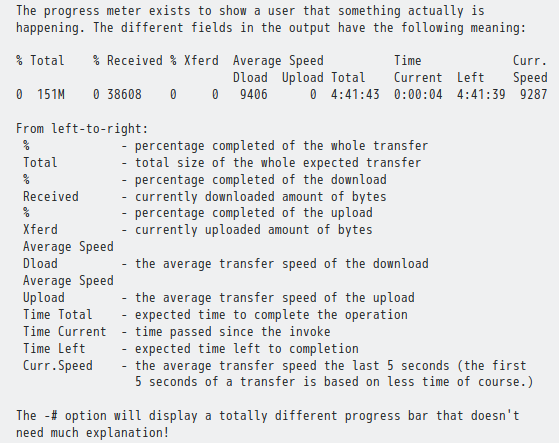
\includegraphics[scale=0.5]{curl-progress-meter}
  \caption{Progress Meter of curl}
  \label{fig:progress-meter-curl}
\end{figure}

To simplify the progress meter, \lstinline|curl| supports
\lstinline|-#| or \lstinline|--progress-bar| option.

Another useful option is \lstinline|-D| that dump the respond
headers to a file for later reference. Cookies from the respond
headers could be read by a second \lstinline|curl| invocation by
option \lstinline|-b, --cookie|. But pay attention to the
\uline{curl CRLF} issue \ref{lst:curl-crlf}. If followed by a dash
\lstinline|-D-|, headers will be dumped to STDOUT.

\subsubsection{curl POST PUT}
\label{sec:curl-post-put}

To post data to a remote server, firstly, we specify the HTTP
request method by \lstinline|-X POST| or
\lstinline|--request POST|. The data to be posted should be
specified by option \lstinline|-d, --data|. \lstinline|curl| will
send the data to the HTTP server in the same way a browser does
when a user has filled in an HTML form and press the submit
button. For example:

\begin{lstlisting}
curl -v -X POST --data 'name=jim' http://www.example.com/api/info
\end{lstlisting}

Data can be loaded from a file, which is done by
\lstinline|-d '@data.file'|. Attention that, the argument is
single-quoted:

\begin{lstlisting}
curl -v -X POST -d '@data.txt' http://223.202.75.26:32000/bm-app/apir/9120/qryLocationInfoAndIp

# data.txt:
name=jim&age=23
\end{lstlisting}

If \lstinline|-d '@-'| is used, then data is read from STDIN:

\begin{lstlisting}
curl -v -X POST -d '@-' http://223.202.75.26:32000/bm-app/apir/9120/qryLocationInfoAndIp
name=jim&age=23
^D
\end{lstlisting}

There are two common data formats, namely ``urlencoded'' and
``JSON'', taking the following two forms:

\begin{lstlisting}
-H "Content-Type: application/x-www-form-urlencoded"

-H "Content-Type: application/json"
\end{lstlisting}

Other formats like XML are not unusual as well. By default,
``urlencoded'' is used as it is concise and neatly organized. So
the ``Content-Type'' header can be omitted. Check this example:

\begin{lstlisting}
curl -v -X POST -H "Content-Type: application/x-www-form-urlencoded" -d 'name=jim&age=23' http://223.202.75.26:32000/bm-app/apir/9120/qryLocationInfoAndIp
\end{lstlisting}

For JSON data, it is recommended to load from external file:

\begin{lstlisting}
curl -v -X POST -H "Content-Type: application/json" -d '@api.json' http://223.202.75.26:32000/bm-app/apir/9120/qryLocationInfoAndIp

curl -v -X POST -H "Content-Type: application/json" -d '{"name": "jim", "age": 23}' http://223.202.75.26:32000/bm-app/apir/9120/qryLocationInfoAndIp
\end{lstlisting}

If the \lstinline|-d| option is supplied multiple times,
\lstinline|curl| will \textit{url-encode} the data before sending
out. \lstinline|--data 'name=jim' --data 'age=23'| will be merged
as \lstinline|'name=jim&age=23'|. It is quite handy for form
fields, though \lstinline|curl| supports option
\lstinline|-F, --form|.

The \lstinline|-d| option has multiple variants like
\lstinline|--data-raw|, \lstinline|--data-urlencode|,
\lstinline|--data-binary| etc. \lstinline|--data-urlencode| is
useful when if the data contain spaces like:

\begin{lstlisting}
curl -v -G "http://localhost:30001/data" --data-urlencode "msg=hello world" --data-urlencode "msg2=hello world2"

# /data?msg=hello%20world&msg2=hello%20world2
\end{lstlisting}

Read more in man page and check
\href{https://gist.github.com/subfuzion/08c5d85437d5d4f00e58}{curl.md}.

\subsection{wget}
\label{sec:wget}

Use \lstinline|wget| to download a remote directory with
\lstinline|-r, --recursive| option:

\begin{lstlisting}
wget -r -l2 -np -R "index.html*,mp3" -nH --cut-dirs=1 http://example.com/dir1/dir2/
\end{lstlisting}

\begin{itemize}
\item \lstinline|-l, --level| specifies the maximum recursion
  depth. By default, it is 5. Value \lstinline|inf| means
  \textit{infinite} recursion.
\item The \lstinline|-np, -no-parent| option does not ever ascend
  to the parent directory when retrieving recursively.
\item An \textit{intex.html} is automatically generated, which can
  be disabled by option \lstinline|-R, --reject| which rejects
  files by \textit{suffix} or \textit{filename}s if wildcard
  characters \lstinline|* ? [ ]| are used. For example,
  \lstinline|-R pdf| excludes PDF files while \lstinline|temp*|
  excludes filenames with leading string \textit{temp}.
\item By default, invoking Wget with
  \lstinline|-r http://fly.srk.fer.hr/| will create a local
  directory beginning with the host
  \textit{fly.srk.fer.hr/}. Option
  \lstinline|-nH, --no-host-directories| removes that.
\item \item \lstinline|--cut-dirs=number| ignores \textit{number}
  directory prefixes.
\end{itemize}

In the example above, \lstinline|-nH, --cut-dirs=1| creates a
local directory \textit{dir2/} without leading
\textit{fly.srk.fer.hr/dir1/} pathname. If we change
\textit{number} to 2, then all files are downloaded in current
directory < \uline{.} >

A similar option is \lstinline|-m, --mirror| to mirror a site. It
is equivalent to \lstinline|-r -N -l inf --no-remove-listing|.

\begin{lstlisting}
wget -m -np -nH --cut-dirs=0 -Epk -R "index.html*,mp3" -X "/video-dir/sexy" [--restrict-file-names=nocontrol] http://192.168.0.105:8080/a/
\end{lstlisting}

\begin{itemize}
\item \lstinline|-E, --adjust-extension| appends suffix
  \textit{.html} to \verb|application/xhtml+xml| or
  \verb|text/html| filenames if it does not end with
  \textit{regex} \lstinline|\.[Hh][Tt][Mm][Ll]?|.
\item \lstinline|-p, --page-requisites| downloads linked resources
  to display a given HTML.
\item \lstinline|-k, --convert-links| converts the links in the
  document to make them suitable for local offline viewing.
\item \lstinline|-X| is to reject unwanted directories, similar to
  \lstinline|-R, --reject|. Please use the full pathname
  \textit{relative} to the URL. \lstinline|-X "/video-dir/sexy"|
  means to exlude
  \textit{http://192.168.0.105:8080/a/video-dir/sexy}. The
  leading forwardslash is optional.
\item \lstinline|--restrict-file-names=nocontrol|. The term
  \textit{restrict} means to allow only characters of filename
  valid and safe to your local operating system. Invalid filename
  characters (including those unprintable control characters) are
  \textit{escaped}. Argument \textit{unix} would escape
  forwardslash \lstinline|/| and unprintable control
  characters. The argument \textit{nocontrol} tells Wget
  \textit{not} to escape control characters. It solves Chinese
  mojibak issue as parts of which fall into the range of control
  characters.
\end{itemize}

\paragraph{Re-downloading of the same pathname} By default,
downloading multiple copies of the same pathname would result in
new copies ending with number suffixes like \textit{pathname.1},
\textit{pathname.2} etc., which is called
\uline{clobbered}. Option \verb|-r| would \uline{overwrite} the
old copy with new one from server. Option \verb|-nc, --no-clobber|
just refuses to download any new copies and \uline{preserve} the
old copy. When option \verb|-N, --timestamping| is used, whether or
not to download a new copy depends on the local and remote
timestamp and size of the file. Remember, do not specify
\verb|-no| and \verb|-N| concurrently. Therefore, either
\verb|-r -nc| or \verb|-r -N|.

\paragraph{To use proxy} \lstinline|wget| supports \lstinline|-e|
option like \lstinline|wget -e https-proxy=127.0.0.1:8080|. Of
course, the proxy setting could set put in \lstinline|/etc/wgetrc|
or \lstinline|~/.wgetrc| like:

\begin{lstlisting}
use_proxy=on

http-proxy=127.0.0.1:8080
https-proxy=127.0.0.1:8080
ftp-proxy=127.0.0.1:8080
\end{lstlisting}

To turn off all proxies, set \lstinline|use_proxy| as
\textit{off}.

\subsection{rsync}
\label{sec:rsync}

We can use \lstinline|rsync| to synchronize files between a source
and a destination. Specially, if one end is an remote host,
\lstinline|rsync| can transfer data over \textit{remote shell}
(\href{https://serverfault.com/q/378939}{default} to
\lstinline|ssh|) or \textit{rsync daemon} (directly over TCP).

If the host is followed by one single colon, \lstinline|ssh|
connection is used. The option \lstinline|-e, --rsh=COMMAND|
specifies the remote shell to use. If it is two colons
(i.e. \lstinline|foo::|) or \lstinline|rsync://|, \textit{rsync
  daemon} is used.

\begin{lstlisting}
# -e "ssh" is optional
# -z compresses contents before transmission, usually used over
# network transmission
rsync -avzP -e "ssh" ~/workspace/src/ dev:~/dev/

# customize SSH port
rsync -avzP -e "ssh -p 2222" ~/workspace/src/ dev:~/dev/

# -n, --dry-run
rsync -n -avzP ~/workspace/src/ dev:~/dev/

# --delete to mirror the source and dest
# If a source file is deleted from the source, then delete it from
# the dest either. By default, only append.
rsync -avzP --delete ~/workspace/src/ dev:~/dev/
\end{lstlisting}

We cannot emphasize too much the paramount importance of trailing
forwardslash \verb|/|:

\begin{itemize}
\item If \verb|/| is placed at the end of the source folder,
  \verb|rsync| will copy the contents of the folder.
\item If the source folder is not followed by \verb|/|,
  \lstinline|rsync| will copy both the folder and contents
  therein.
\item If \verb|/| is palced at the end of the target folder,
  \lstinline|rsync| will paste the data directly inside that
  folder.
\item If the target folder is not followed by \verb|/|,
  \lstinline|rsync| will create the target folder and then paste
  the data inside.
\end{itemize}

\subsection{tr}
\label{sec:bash-tr}

Command \lstinline|tr| translates, squeezes, \uline{and/or}
deletes characters from standard input, writing to standard
output. It takes form as:

\begin{lstlisting}
tr [OPTION]... SET1 [SET2]
\end{lstlisting}

\uline{SET1} and/or \uline{SET2} define ordered sets of characters
like \lstinline|[:alpha:]| and \lstinline|c-g| (without
brackets). The format of the SET1 and SET2 arguments resembles the
format of regular expressions \ref{cha:regular-expression};
however, they are not regular expressions, only lists of
characters.

The \lstinline|-c -C --complement| option replaces SET1 with its
complement (all of the characters that are not in SET1). Currently
\lstinline|tr| fully supports only single-byte characters. So
characters like Unicode Chinese are not supported.

\textit{translate} means to substitute each character of its input
that is in SET1 to the \textit{corresponding} character in SET2
(required). Therefore, we usually want the lengths of both sets
are equal.

To replace comma with newline \lstinline|tr ',' '\n' < file|. It
is quite handy though we can do that with \lstinline|sed| or
\lstinline|awk|.

A common use of \lstinline|tr| is to convert lowercase characters to
uppercase.

\begin{lstlisting}
tr abcdefghijklmnopqrstuvwxyz ABCDEFGHIJKLMNOPQRSTUVWXYZ

tr a-z A-Z # discouraged method

tr '[:lower:]' '[:upper:]'
\end{lstlisting}

The bare range \verb|a-z| and \verb|A-Z| are discouraged as it is
not portable and depends on implementation.

Option \lstinline|-d| deletes characters in \uline{SET1} and do
\textbf{not} \textit{translate}. For example
\lstinline|tr -d '\0'| removes all zero bytes.

\lstinline|-s| can be treated as a special case of \lstinline|-d|,
which \textit{squeeze}s repeated occurence. For example,
\lstinline|tr -s '\n'| merge multiple blank lines to a single one.

Let's have a look at:

\begin{lstlisting}
tr -d -axM # fail

tr -d -- -axM
tr -d axM-
tr -d '[=-=]axM'
\end{lstlisting}

The code want to delete four characters in which hyphen is
included. In the first case, \lstinline|-a| will be treated as
command-line option. The last method uses \textit{equivalence
  class}. For details, check the \lstinline|info tr| page.

\subsection{dig}
\label{sec:bash-dig}

The \lstinline|+trace| option traverses the resolution system in a
\textit{iterative} resolution method. At the very first, local
name server (i.e. \textit{/etc/resolv.conf} is used to obtain a
list of root domain name server unless \lstinline|@name-server| is
specified. For example:

\begin{lstlisting}
# dig +trace www.bing.com. @1.2.4.8
\end{lstlisting}

\section{Math}
\label{sec:bash-math}

\href{http://mywiki.wooledge.org/ArithmeticExpression}{Arithmetic}
in Bash is \textit{integer} math only. To do floating point math,
resort to \textit{bc} command.

We call a \textit{math form} as \textit{math context}. The basic
math form is
\lstinline|$(())| with the complete syntax at
\href{https://wiki.bash-hackers.org/syntax/arith_expr}{arith expr},
which is called \uline{Arithmetic Expansion}. Basically, within a
math context, we use the same syntax as C language like.

\begin{minipage}{1.0\linewidth}
\begin{lstlisting}
# POSIX sh
i=$((j + 3))
lvcreate -L "$((24 * 1024))" -n lv99 vg99
q=$((29 / 6)) r=$((29 % 6))
if test "$((a%4))" = 0; then ...
echo "$((2**3))"
\end{lstlisting}
\end{minipage}

Within a math context, pay attention to the concept of the
\textit{evaluation value} of each \textit{arithmetic expression}
and the value returned to the Bash environment by the context
itself (name it \uline{context value}?).

\begin{itemize}
\item All C arithmetic operators are supported, including
  \verb|?:|. Bash brings in \textit{exponentiation} operator
  \verb|**|.
\item Within a single math context, multiple expressions can be
  separated by \textit{comma}. Value of the last expression
  becomes that of the math context.
\item Variable \textit{name} in a math context are substituted
  with their values (unset or empty variables are evaluated as
  0). There is no need to use parameter expansion
  (i.e. \verb|${i}|) within math context.
\item Numbers without leading 0 are treated as base 10. Numbers
  with a leading 0x are treated as base 16. Numbers with a leading
  0 (not followed by x) are treated as base 8.
\end{itemize}

\subsection{Arithmetic Command}
\label{sec:bash-arithmetic-command}

Besides, Bash offers two extra forms of math context by
\textit{commands} for which, the math context \textit{also} gets
an exit status, and side effects. Similar to arithmetic expression
\lstinline|$(())|, the context value of an arithmetic command is
that of the command exit code.

Exit code of arithmetic command \uline{depends on but not equal
  to} evaluation value of the last expression. If the
expression evaluates to 0 and the command is considered a falure. To
be logically consistent with Bash, the command returns 1
. Otherwise, the command is regarded successful and return
0.

Consequently,

\begin{itemize}
\item Evaluation and boolean logic (0 false, non-zero true) of
  math expressions are in accord with C syntax.
\item Exit code and boolean logic (0 true, non-zero false) of math
  commands are in accord with Bash.
\item Return eithr 0 or 1. Nothing else. This is different to the
  Arithmetic Expansion above. So we can the Arithmetic Command as
  a \lstinline|test| with \lstinline|for| or \lstinline|while|.
\item Please go back and read Exit Codes and Boolean
  \ref{sec:exit-codes-boolean}.
\item Whatever numeric values are involved, boolean logic must be
  guaranteed. This is the rule that we follow when
  scripting. Forget about the details then. Check
  \href{https://wiki.bash-hackers.org/syntax/arith_expr#arithmetic_expressions_and_return_codes}{Arithmetic
    expressions and return codes}.
\end{itemize}

The first arithmetic command is \lstinline|let|:

\begin{minipage}{1.0\linewidth}
\begin{lstlisting}
let a=17+23
echo "a = $a"        # Prints a = 40
#
let a=17 a+=23 a=0   # the last expression evaluates to 0
echo $?              # 1 (false)
#
let a[1]=1+1         # Wrong (if a1=1+1 exists or shopt -s failglob)
( shopt -s failglob; let a[1]=1+1 )
touch a1=1+1; let a[1]=1+1; declare -p a
let 'a[1]=1+1'       # right
\end{lstlisting}
\end{minipage}

Note that each arithmetic expression has to be passed as a single
argument to the \lstinline|let| command, so you need quotes if
there are spaces or globbing characters.

\lstinline/let a[1]=1+1/ is not right as \lstinline|[ ]| are
\href{http://mywiki.wooledge.org/glob}{glob} characters, which
matches one and only one of the enclosed characters like regular
expression.

\begin{quotation}
  Bash expands globs which appear \textit{unquoted} in commands,
  by matching \textit{filenames} relative to the current
  directory. The expansion of the glob results in 1 or more words
  (0 or more, if certain options are set), and those words
  (filenames) are used in the command.
\end{quotation}

So Bash tries to expand \lstinline|a[1]=1+1| as filename
\textit{a1=1+1} before \lstinline|let| is executed. If that file
exists or \textit{failglob} is turned on, Bash reports:

\begin{quotation}
  bash: no match: a[1]=1+1
\end{quotation}

Now let's move on to the next arithmetic command
\lstinline|(( ))|. It resembles Arithmetic Expansion but removes
the leading dollar
\lstinline|$| sign. It is identical to \lstinline|let| but does
not require quotes since expressions inside are delimited by
Bash metacharacters \lstinline|(| and \lstinline|)|.

\begin{lstlisting}
((a=$a+7))         # Add 7 to a
((a = a + 7))      # Add 7 to a.  Identical to the previous command.
((a += 7))         # Add 7 to a.  Identical to the previous command.

((a = RANDOM % 10 + 1))     # Choose a random number from 1 to 10.
echo $?                     # % is modulus, as in C.

echo "$(( a = RANDOM % 10 + 1 ))" # becomes Arithmetic Expansion
\end{lstlisting}

Specially, we can compare integers with
\lstinline|(())|. \lstinline|>| or \lstinline|<| inside
\lstinline|(( ))| means greater/less than, not output/input
redirection involved. Recall that I have talked about expression
evaluation and context exit code above. Integer comparision
expression also follows the same rules.

The only difference is that arithmetic expression within the
command is logic operation: only evaluates to 1 or 0. If the
comparison is true (command executes successfully), the expression
evalutes to 1 and returns 0. If it is false, the expression
evaluates to 0 and returns 1.

\lstinline|(( ))| is used more widely than \lstinline|let|,
because it fits so well into an \lstinline|if| or
\lstinline|while| command like

\begin{lstlisting}
if (( $# > 2 )) ; then printf 'there are more than 2 arguments\n'; fi
\end{lstlisting}

\subsection{bc calculator}
\label{sec:bc-calculator}

To do \href{http://mywiki.wooledge.org/BashFAQ/022}{floating point
  calculation}, we use \lstinline|bc|. However, by default, it
truncates according to the \textit{scale} argument instead of
rounding.

We increase \lstinline|scale| and pass the result to
\lstinline|xargs printf| like:

\begin{lstlisting}
bc <<< 'scale=3; 7/242.906' # 0.028
bc <<< 'scale=2; 7/242.906' # 0.02

bc <<< 'scale=3; 7/242.906' | xargs printf "%.2f\n" # 0.03
\end{lstlisting}

Another possible workaround is to use \verb|±0.5| trick with the final
result like:

\begin{lstlisting}
rounding()
{
    if (( $(bc <<< "$1 < 0") )) ; then offset=-0.5 ; else offset=0.5; fi
    printf "%.$2f\n" "$( bc -l <<< 'scale=$2; (((10^$2)*$1)+$offset)/(10^$2)' )"
    printf '%.*f\n' "$2" "$( bc -l <<< 'scale=$2; (((10^$2)*$1)+$offset)/(10^$2)' )"
}
\end{lstlisting}

Within the rounding function, we should set the offset according
to the sign of the number. If the number is negative, we choose to
round it toward the left side of number line. Or we can say to
round toward its absolute value. Of course, if we want to always
round toward the right side, then just use \verb|0.5|.

About \lstinline|printf '%.*f\n' "$2"|, the asterisk means the width
is given as argument
\href{https://wiki.bash-hackers.org/commands/builtin/printf?s\%5b\%5d=printf}{before}
the string or number is printed.

\section{Redirection}
\label{sec:bash-redirection}

Redirection takes the form as \verb|lhs op rhs|, which can
\textit{open}, \textit{duplicate}, \textit{move} or we want to
\textit{close} file descriptors.

\begin{itemize}
\item \textit{lhs} is always a file descriptor, namely an integer
  like \verb|0|, \verb|1|, \verb|2|, or \verb|3|. If the
  \textit{op} is \verb|<| then there is an \textit{implicit}
  \verb|0| as \verb|0<|. If it's \verb|>| or \verb|>>|, there is
  an \textit{implicit} \verb|1| as \verb|1>| or \verb|1>>|.
\item \textit{op} is \verb|<|, \verb|>|, \verb|>>|, \verb/>|/, or
  \verb|<>|. Two special redirections \verb|<<| (here document)
  and \verb|<<<| (here string) usually require string(s) for
  \textit{rhs}. Details, read the official manual.
\item \textit{rhs} is the thing that the file descriptor will
  describe. It can be a filename, or the place where another
  descriptor goes ( prefixed with \verb|&| like \lstinline|&1|),
  or \lstinline|&-| that will close the \textit{lhs} file
  descriptor.
\end{itemize}

When redirection is used, the \textit{lhs} is pointed to what
\textit{rhs} is \textbf{currently} pointed to. If, later on,
\textit{rhs} is pointed to another place, \textit{lhs} remains and
won't follow \textit{rhs}'s update. We can think of a file
descriptor as C language pointer.

To check which place file descriptors are currently pointed, we
can:

\begin{lstlisting}
ll /proc/$$/fd/

# total 0
# dr-x------ 2 outsinre outsinre  0 Feb 14 15:49 .
# dr-xr-xr-x 9 outsinre outsinre  0 Feb 14 15:49 ..
# lrwx------ 1 outsinre outsinre 64 Feb 14 15:49 0 -> /dev/pts/2
# lrwx------ 1 outsinre outsinre 64 Feb 14 15:49 1 -> /dev/pts/2
# lrwx------ 1 outsinre outsinre 64 Feb 14 15:49 2 -> /dev/pts/2
# lrwx------ 1 outsinre outsinre 64 Feb 14 21:10 255 -> /dev/pts/2

for fd in 0 1 2 255; do cat /proc/$$/fdinfo/$fd; echo; done
\end{lstlisting}

In the following code, \textit{cmd} reads input from filename
\textit{myFile}. File descripted \verb|3| is associated with
\verb|1| (standard output, \textit{/dev/pts/2}). But the script
does not make use of the new descriptor. \verb|2| (standard error,
\textit{/dev/pts/2}) is redirected to
\lstinline|/dev/null|. Standard output (implicit \verb|1|,
\textit{/dev/pts/2}) is redirected to \verb|2|, which is now
pointed to \textit{/dev/null}.

\begin{lstlisting}
# Good! This is clearly a simple commmand with two arguments and 4 redirections
cmd arg1 arg2 <myFile 3<&1 2>/dev/null >&2
\end{lstlisting}

There are two special redirection forms \lstinline|fd1>&fd2| and
\lstinline|fd1<&fd2|. As mentioned earlier, if \textit{fd1} is
omitted, the default value are \verb|1| and \verb|0|
respectivelly.

They are called \textit{descriptor copy} or \textit{descriptor
  duplication}. Technically speaking, the two forms \textbf{make no
  difference}. Yeah, they are equal in Bash grammar except the
different implicity \textit{lhs}.

\textit{fd1} is opened (created) if it does not exist, and pointed
to where \textit{fd2} is currently pointed. Whether \textit{fd1}
is opened for reading or writing, depends on \textit{fd2}. If the
file \textit{fd2} linked with is on read mode, then we can use
\textit{fd1} for reading. Similarly, we can write to \textit{fd1}
when \textit{fd2} points to a file on write mode. Obviously, if
the file is on read/write mode, \textit{fd1} can be used to read
from and write to that file.

In a script, we can do like this:

\begin{lstlisting}
exec m>&n
exec m<&n
# -or-
cmd arg1 arg2 m>&n
cmd arg1 arg2 m<&n
\end{lstlisting}

It is necessary to tell apart \verb|>, <| and \verb|>&, <&| as the
\verb|&| requires an integer descriptor followed while the former
needs a filename. More importantly, \verb|>, <| cares about the
read and write mode. \verb|>| opens a file descriptor for writing
(\uline{redirecting output}). The other one for reading
(\uline{redirecting input}). Apparently, \verb|>>| is for
\uline{appending redirected output}.

To open a file descriptor for both reading and
writing, we can:

\begin{lstlisting}
[n]<>word

exec 3<>/path/to/filename
\end{lstlisting}

If \textit{n} is omitted, it defaults to 0. If the filename of
\textit{word} expansion does not exist, it is created.

Sometimes, we need to store the integer value in a variable. Then
enclose it with braces:

\begin{quotation}
  Each redirection that may be preceded by a file descriptor
  number may instead be preceded by a word of the form
  \verb|{varname}|. In this case, for each redirection operator
  except \verb|>&-| and \verb|<&-|, the shell will allocate a file
  descriptor greater than or equal to 10 and assign it to varname.
  If \verb|>&-| or \verb|<&-| is preceded by \verb|{varname}|, the
  value of varname defines the file descriptor to close.
\end{quotation}

\begin{minipage}{1.0\linewidth}
\begin{lstlisting}
fd=0; echo "hello, world" >> /tmp/foo; exec {fd}</tmp/foo;
printf '%d\n' $fd
read -r -u "$fd" line; printf '%s\n' "$line"
\end{lstlisting}
\end{minipage}

We can also \textit{move} a file descriptor, which first duplicate
the \textit{rhs} and then close it.

\begin{lstlisting}
[n]<&digit-
[n]<&digit-

m<&n-; m>&n-
<&4-; 0<&4-
>&4-; 1>&4-
\end{lstlisting}

Read more at \href{https://unix.stackexchange.com/q/42728}{Switch
  stdout and stderr},
\cprotect{\href{https://unix.stackexchange.com/a/18904}}{What does
  \verb|3>&1 1>&2 2>&3| do in a script} and
\href{https://unix.stackexchange.com/q/131801}{Closing a file
  descriptor, \texttt{>\&} vs. \texttt{<\&-}}.

\section{Set or Not}
\label{sec:set-or-not}

It happens when we want to test
\href{https://stackoverflow.com/a/13221491}{whether a \textit{name}
  is set or not}. Just use:

\begin{lstlisting}
[[ "${array[key]+abc}" ]] && echo "exists"
\end{lstlisting}

This code applies to both indexed and associative
array. \lstinline|"${array[key]+abc}"| is actually a
\uline{special} form of parameter expansion with the colon
omitted. The original form is
\lstinline|${parameter:+word}|. From the manual, we find:

\begin{quotation}
  if the colon is omitted, the operator tests only for existence [of parameter] 
\end{quotation}

\begin{itemize}
\item if \lstinline|array[key]| is set, return \textit{abc}.
\item if \lstinline|array[key]| is not set, return nothing
\end{itemize}

However, we still can add the colon but the substitution procedure
is carried out, though that does not affect the logic.

\begin{lstlisting}
# degrade performance

[[ "${array[key]:+abc}" ]] && echo "exists"
\end{lstlisting}

Another method is to use built-in \textit{test} option
\verb|-v VAR|:

\begin{quotation}
  -v VAR         True if the shell variable VAR is set.
\end{quotation}

When to check for existence in this method, do \textbf{not} use
parameter expansion. The name itself is enough.

\begin{lstlisting}
[[ -v ar["hello"] ]] && echo "exists"
declare a=1; [[ -v a ]] && echo "exists" || echo "no"

declare -A ar=( [0]=1 ['b c']=2 ); [[ -v ar ]] && echo "yes"
declare -A ar=( [a]=1 ['b c']=2 ); [[ -v ar[@] ]] && echo "yes"
\end{lstlisting}

The first two lines test whether a name set.

The third tests the key of \verb|0|. In the 4th case, the bare
\verb|a[@]| (without
\verb|$| prefixed) is \textbf{not} a parameter expansion and hence
it does \textbf{not} expand to postional index. This code tests
for any array element. If there exists at least one element set,
then exits true.

A different version is:

\begin{lstlisting}
# test var
_regex="^declare -[aA] ${var}[=|$]"
[[ "$(declare -p $ar)" =~ "${_regex}" ]] && echo "yes"
\end{lstlisting}

Here is a function to test whether a specific value is stored in
array. It is mainly for index arrays. If it is an associative
array, just use the corresponding key to test.

\begin{lstlisting}
#!inarray
# Usage: inarray "$value" "${array[@]}"
inarray() { local n=$1 h; shift; for h; do [[ $n = "$h" ]] && return; done; return 1; }
\end{lstlisting}

\section{String as Delimiter}
\label{sec:bash-str-as-delim}

To split string with just a single delimter, we just need
\lstinline|read| command and \lstinline|IFS| variable.

In the section \ref{sec:bash-awk}, \lstinline|mapfile|,
\lstinline{awk}, and \textit{process substitution} are used to
split a string with another string. I will introduce
\href{https://www.tutorialkart.com/bash-shell-scripting/bash-split-string/#split-string-with-multiple-character-delimiter}{Split
  strings with group delimiters} in this section.

\begin{minipage}{1.0\linewidth}
\begin{lstlisting}
_headers_sep=')@|#('
_headers_regex=$'\^\~\$headers=\'(.*)\)@\|#\(\'' #'

tmp_headers="${BASH_REMATCH[1]}${_headers_sep}" _headers_array=()
while [[ -n $tmp_headers ]]
do
    _headers_array+=( "${tmp_headers%%${_headers_sep}*}" )
    tmp_headers="${tmp_headers#*${_headers_sep}}"
done; unset tmp_headers
\end{lstlisting}
\end{minipage}

We define the string delimiter as \lstinline|_headers_sep|. When
doing the parameter expansion, there is no need to escape those
characters as \lstinline|_headers_regex| does.

\section{signal(7)}
\label{sec:signal7}

POSIX signals are classified into \textit{reliable signals} and
\textit{real-time signals}. Reliable signal, hereinafter, is
called \textit{standard signal}.

Each signal has a default \textit{disposition} that determines the
\uline{action} to perform when the process is delivered the
signal. For instance, Action \uline{Term} terminates a process and
action \uline{IGN} ignores the process etc. However, a process can
change the default by \textit{sigaction(2)} or
\textit{signal(2)}. The signal disposition is a
\textit{per-process} attribute: in a multithreaded application,
the disposition of a particular signal is \textit{the same} for
all threads.

Some system calls or library functions allow the caller to
\textit{send} a signal like \uline{kill(2)} and \uline{raise(3)};
other system calls and library functions suspend execution of the
calling process or thread until a signal is caught
(\textit{receive} a signal) like \uline{pause(2)} and
\uline{sigsuspend(2)}.

A signal takes the form of an upper case string
(i.e. \uline{SIGTERM}) or an integer (i.e. \uline{15}). The fixed
prefix \uline{SIG} can be removed (i.e. \uline{TERM}). Standard
signals like \uline{SIGHUP 1}, \uline{SIGINT 2}, \uline{SIGKILL
  9}, \uline{SIGTERM 15} and \uline{SIGSTOP 19} are often used
when doing system operation.

\uline{SIGHUP} tells a process to reload configuration
files. \uline{SIGINT} sends a terminal interrupt signal by
\verb|Ctrl-C| to terminate a process. Similarly, \verb|Ctrl-Z|
suspends execution. \uline{SIGTERM} also terminates a process but
it can be caught (and interpreted) or ignored, allowing a graceful
termination by releasing resources and saving
states. \uline{SIGTERM} is almost identical to \uline{SIGINT,
  Ctrl-C}. \uline{SIGKILL} terminates a process immediately (kill)
in a brute force way. It cannot be caught or ignored, and the
receiving process cannot perform any clean-up upon receving the
signal: the \textit{last} resort to terminate a process. The
\uline{SIGSTOP} tells the operating system to \textit{stop} a
process for later resumption by \uline{SIGCONT}.

Linux provides the \lstinline|kill(1)| command line (the user
interface of \uline{kill(2)} system call) to send a signal to a
process. \lstinline/kill [-l | -L]/ lists available
signals. Without specifying the signal, \uline{SIGTERM} is
sent. The following three lines are equivalent:

\begin{lstlisting}
kill [-s | --signal] -<signal> <pid1> <pid2> [...]

kill -15 12345
kill -SIGTERM 12345
kill -TERM 12345
\end{lstlisting}

Recall that, the 3rd column of \lstinline|ps -eF| command prints
the parent process ID (PPID or GPID). To send a signal to the
process group, prefix the GPID with a \textit{minus} symbol. A
GPID of \verb|-1| is special as it indicates all processes except
the kill process itself and \textit{init}.

% ARRAY line
% MAPFILE _log_array
% channel msg
% for f in full real; do declare "_$f"="${_log_time}_${_num_of_tests}_$f.log"; done
% log_time='midnight'; num_of_tests=99;  declare -A fn=();  for f in full real; do  fn[$f]=$log_time-$num_of_tests-$f.log;  done;
% if you ever feel need for automatical generation of names for variables in bash, it means you need to approach your problem using associative array
% sep=')@|#('; data='hello)@|#(there)@|#(blah)@|#('; readarray -t split <<<"${data//"$sep"/$'\n'}";  declare -p split
% eval vs exec https://unix.stackexchange.com/a/296852
% https://www.cnblogs.com/cyfonly/p/5800758.html
% awk 'FNR==NR{a[$0]=$1;next} $1 in a{print $0}' file-a file-b > file-c
% difference between nohup, disown and & https://unix.stackexchange.com/a/148698


\lstset{language=TeX}

%%% Local Variables:
%%% mode: latex
%%% TeX-master: "main"
%%% End:
